\chapter{coupes divinatoires}



 

\section{Annexe : références}


\subsection{Coupes achetées}


\paragraph{Coupe divinatoire} dit bol \textit{magique} en alliage de cuivre partiellement étamé, de forme circulaire aux bords évasés. La paroi extérieure est gravée d'une fleur de lotus à huit pétales calligraphiés au coeur en forme d'une étoile à cinq branches, et une longue inscription le long du rebord externe. L'intérieur est décoré d'un cartouche inscrit, de deux motifs de tughra, d'un sceau de propriétaire en forme d'amande «sahib Tador (Théodore ?) «et d'un cachet ARMENIEN daté 1875». Le rebord est gravé d'une longue frise épigraphique sur deux lignes. Empire ottoman, datée 1875.
Haut. : 4,9 ; Diam. : 15,1 cm
\begin{figure}[h!]
    \centering
        \sidecaption{Coupes divinatoires}
 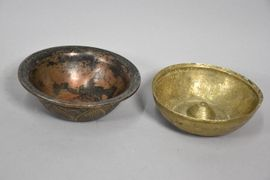
\includegraphics[width=\textwidth]{GénéralISTR/Image/bolsmagiques.jpeg}

%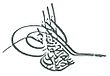
\includegraphics[]{GénéralISTR/Image/Tughra_of_Abdülaziz 1861-76.jpeg}

    \label{fig:my_label}
\end{figure}


\paragraph{fleur de lotus} Dans le bouddhisme, le lotus est associé à la pureté, à l’éveil spirituel et à la fidélité. La fleur est considérée comme pure car elle est capable de sortir des eaux troubles le matin et d’être parfaitement propre. Il est également connu pour symboliser la pureté de la parole, du corps et de l’esprit.


\paragraph{Bol talismanique ou bol magique} coupe de forme circulaire à bords évasés, ombiliquée en laiton anciennement étamé incrustation de pâte noire gravé à l'intérieur de mihrabs, inscriptions en écriture naskh\sn{Le naskh, aussi appelé naskhi ou neskhi  est le style d'écriture le plus répandu pour les langues utilisant l'alphabet arabe. C'est ce style que l'on apprend à l'école et que l'on emploie pour la calligraphie et l'écriture usuelle, manuscrite ou imprimée.} et nasta'liq\sn{Le nastaliq    est un des styles de la calligraphie persane, en alphabet persan, dont l'origine est attribuée à Mir Ali Tabrizi, originaire de Tabriz, au xive siècle} d'invocation religieuse et verset coranique, patine d'usage. Iran XIX-XXe.
Haut. : 4 ; Diam. : 13,5 cm


\paragraph{Classical Islamic Theology}\sn{Tim Winter. The Cambridge Companion to Classical Islamic Theology (Cambridge Companions to Religion) (pp. 188-189). Cambridge University Press. Édition du Kindle. } \cite{winter_cambridge_2008}
\begin{quote} 
    That its signifier is such an important part of its signified contributes in making the Qur’an a much richer reality than a mere book to be read and studied. Of course, even before being a scripture, the revelation sent down to Muammad is a speech. And as God Himself explains, the words of this speech operate in many ways. They are not supposed to affect minds only. “They only are the believers whose hearts tremble with fear when God is mentioned. When His verses are recited to them, they make their faith increase and they put their trust in their Lord” (8:2). “When the verses of the Compassionate are recited to them, they fall down in prostrate adoration, weeping” (19:58). “God has sent down the most beautiful speech as a Scripture … whereat the skins of those in awe of their Lord shiver, and then their skins and their hearts soften to God’s remembrance” (39:23). “We send down, as the Qur’an, something that is a healing and a mercy for the believers” (17:82). This healing power of the revelation is understood literally by many, not just spiritually. The qur’an was thus sometimes also used physically for curing ailments: a piece of paper with a qur’anic inscription was dipped into water; once the ink was diluted, the qur’anically enriched water was drunk. By means of amulets, talismanic shirts and other artefacts covered with qur’anic inscriptions, often in conjunction with astrological or magical devices or practices, the revelation came to be put to all kinds of uses, not always strictly orthodox. By procedures reminiscent of the Cabbala, the letters of the Arabic alphabet and their numerical values themselves played an important role in Muslim mysticism, esotericism and the divinatory arts. This is particularly true of the seventy-eight “mysterious” letters opening twenty-nine of the qur’anic sūras (2–3, 7, 10–15, 19–20, 26–32, 36, 38, 40–6, 50, 68) and which, once they are reduced to the fourteen of which they are combinations, represent the various basic consonantal forms of written Arabic, hence of the whole Arabic alphabet.11 The fact that through qur’anic psalmody and calligraphy the most manifest ways of celebrating God’s revelation have given rise to arts that are among the most representative of Islam, if not the two major Islamic arts, is also to be explained as an aspect of what the Algerian Malek Bennabi rightly called “the Qur’anic phenomenon”. Be it through architecture, decorative arts, the media or other aspects of everyday life, the divine revelation conveyed in Arabic by the Prophet continues to be as present in the public sphere as it is in the hearts of the millions of those who, in their childhood, learn it by heart, often entirely. And just as Arabic is per se part of the Qur’an, the latter impregnates it to the point of making it impossible for non-Muslim Arabic-speakers not to be, in some way, linguistically Islamised.
 


\end{quote}


\begin{quote}
    La mise en scène du pouvoir au Moyen Âge confère aux souverains une autorité de nature quasi magique. Aziz Al-Azmeh dépeint ainsi la figure idéale de
l’homme de pouvoir dans l’Islam médiéval :
\begin{quote}
    Au niveau le plus élémentaire, n’importe qui aurait commencé avec les
qualités quasi-magiques de la personne du calife. Il y a un propos, très
répandu dans les écrits arabes médiévaux et attribué à la sagesse persane,
selon lequel la justice d’un roi – sulṭān, un terme fréquemment appliqué
aussi aux califes – garantit le bon fonctionnement des saisons, la
pluviosité et l’irrigation idoine, la bonne reproduction du bétail et le fonctionnement
correct du commerce. Cette indication n’est pas simplement
réductible à une expression sur les connections structurales du monde de
la prospérité détaillée dans le ‘cercle de justice’ étudié dans le précédent
chapitre, mais a des interprétations au-delà et en-deça de celles de la sagesse
politique et des conseils généraux aux rois. Il était perçu comme une
manifestation empirique que l’injustice royale ne produit pas seulement
des effets matériels délétères, mais suscite des forces surnaturelles qui
agissent ineffablement, à une certaine distance, en faisant arrêter le ciel
de pleuvoir et le bétail de se reproduire. Les effets naturels de l’injustice
royale ne sont pas simplement métaphoriques, parce qu’ils ont à faire 
 avec la baraka selon deux aspects alambiqués : la baraka obtenue avec la
justice, qui se tarit avec l’injustice. La baraka était bien sûr partagée avec
les cheikhs soufis et les saints ḥanbalites. De nombreux actes et capacités
merveilleux et tangibles étaient attribués à Aḥmad b. Ḥanbal et d’autres ;
\end{quote}


mais ceux-ci étaient aussi recherchés du lointain calife1.
Ainsi les sujets étaient en droit d’attendre la justice du pouvoir politique, et
la justice est elle-même une condition préalable pour la bénédiction dont
peuvent bénéficier les sujets. Le souverain devait rivaliser avec les saints en
justice et en bienveillance. Il était supposé avoir – dans la mesure du possible –
la capacité de prévenir les sinistres. L’intérêt des cours pour la magie et la divination
avait une réelle signification politique. L’existence de copies du Šams
al-maʿārif dédicacées à des figures politiques, comme nous allons le voir, est un
indicateur important dans cette perspective.\cite{coulon_magie_2017}
\end{quote}
\paragraph{Duquoc} Nous nous trouvons là devant une ferme conviction :

\begin{quote}
    « Jésus ne se replie pas sur l’instant, il l’ouvre à sa profondeur », car le présent est « l’habitat de Dieu » (p. 113).
\end{quote} 
L’auteur revient sur ce point avec insistance, comme pour surmonter le caractère paradoxal des affirmations du Christ, puisque si le Règne est là, le mal et l’injustice, eux aussi, semblent continuer de régner, inexorablement. La « tentation » est alors grande de vouloir faire coïncider le Règne présent avec la fin d’une histoire réconciliée qui dénie les réalités de notre histoire souffrante, en faisant appel à la \textbf{magie}, à la puissance messianique, à la conquête instaurant de force l’unité du Règne promis (comme le suggère le tentateur à Jésus au seuil de sa mission). L’Église n’a pas toujours résisté à cette tentation, comme on le voit lorsqu’elle cherche à dominer et à orienter la politique, illusion dénommée chrétienté (l’auteur développe ici sa réflexion en tirant profit du livre de Marcel Gauchet : La religion dans la démocratie. Parcours de la laïcité, Gallimard, Paris, 1998).  

\subsection{Dictionnaire sociologie religions}

 \paragraph{du prophétisme }
 
Du latin divinatio, deviner, le terme « divination » désigne l'action qui se donne pour objectif de deviner, prévoir et/ou influencer une réalité cachée, à l'aide de la lecture d'éléments, ou présages, selon une technique particulière impliquant leur observation ou leur manipulation. Ainsi définie, la divination apparaît comme une pratique universelle des sociétés  Les procédures divinatoires peuvent être motivées par diverses raisons découvrir les causes d'une maladie ou d'une infortune, retrouver un objet perdu, connaître les déterminations pesant sur l'avenir proche (dans le domaine de l'amour, du travail, etc.), être informé des circonstances propices à la réalisation d'une action ainsi que de ses chances de succès (départ à la guerre ou à la chasse, construction d'une maison, installation sur un territoire, etc.). La divination peut aussi être exécutée de manière quasi automatique, parce qu'elle est requise en telle circonstance par la tradition ou qu'elle fait partie intégrante d'un rituel. La divination est, soit explicative   et renvoie alors à des éléments passés, soit prédictive permettant de
connaître l'avenir de sorte à agir en conséquence. Elle peut être réalisée pour le compte d'un individu, d'un groupe, ou d'un « bien » (du bétail, par exemple).
Les éléments qui servent de présages sont variés et leur lecture est susceptible d'être effectuée selon des procédés très divers : observations et/ou manipulations d'entrailles d'animaux sacrifiés, de vols d'oisceaux, de craquelures sur une carapace de tortue calcinée, de marc de café, de combinaisons d'objets lancés, de cartes, de présence de taches dans un jaune d'œuf, de l'emplacement des planètes, etc. Cette multiplicité des techniques s'illustre par la diversité des termes formés à partir de la racine grec \textit{mantiké} -divination-pour les désigner : chiromancie, géomancie, cartomancie, etc. La divination peut aussi être opérée sans autre support que le devin lui-même. Elle s'inscrit alors plutôt dans le domaine de la voyance : le devin établit un contact qui est dit direct -via les rêves, la transe ou la possession- avec des forces sur-naturelles. Mais si de multiples classifications des formes de divination ont été proposées formes ou techniques intuitives, inspirées, inductives, raisonnées..), aucune n'apparaît universellement pertinente, et il semble plus utile de se référer aux classifications indigènes
- les modes de divination étant généralement pluriels dans une même société.

\paragraph{Hasard exclu des évènements}
En se fondant sur la combinaison, qui
nés à semble résulter du hasard, des éléments qui tion- servent de présages, la procédure divinatoire incie, manipule l'aléatoire pour mieux le dépasser.
si être
Une signification étant attribuée à chacune
 des combinaisons possibles. le hasard est   exclu de la trame des événements. L'incertitude qui motive la divination se trouve alors   intégrée dans un ordre intelligible et
  rassurant.

 le cours du destin peut toujours être plus ou moins « forcé ». Les processus divinatoires prédictifs servent d'ailleurs souvent à se prémunir contre un événement futur potentiel, voire à créer un autre futur : il est fréquent de recommencer une divination jusqu'à obtenir le résultat escompté, comme s'il s'agissait de mettre en place les conditions propices à la réussite de l'action que l'on souhaite entre-prendre. De ce fait, la divination intéresse les réflexions sur les processus de prise de décision et les théories de l'action. Entérinant certaines formes d'actions, elle œuvre comme une procédure de validation, ce qui la rapproche des systèmes juridiques.
\paragraph{Individuel et social}
La divination relève en fin de compte autant de l'individuel que du social. Elle est le résultat d'une interaction, impliquant au minimum le devin et son client, et généralement tout un pan de la société. En inscrivant le destin individuel dans un ordre englobant, les processus divinatoires font de l'individu un élément d'un système socio-cosmique qui le dépasse. Entre l'individu et le social, l'aléatoire et la détermination, l'interprétation et l'action, le religieux et le juridique, les processus divinatoires, variés dans leurs formes et leurs fonctions, touchent à de nombreux aspects de la vie d'une société, qu'ils permettent d'articuler.

\paragraph{bibliographie}
\begin{itemize}
    \item ADLER A. et ZEMPLENI A., Le Bâton de l'aveugle : divination, maladie et pouvoir chez les Moundang du Tchad, Paris, Hermann « Savoir », 1972.   
    \item  CAQUoT A.
et LEIBOVICI M. (éds), La Divination, Paris, PUF,
1968. - EVANS-PRITCHARD E. E., Sorcellerie, oracles et magie chez les Azandé (1937), traduction ft. L.
 Evrard, Paris, Gallimard, 1972. 

  \item  FAHD T., La Divination arabe: études religieuses, sociologiques et folkloriques sur le milieu natif d'Islam, Leyde, Brill, 1966. \href{https://books.google.fr/books?id=ETsVAAAAIAAJ&lpg=PP1&hl=fr&pg=PA8#v=onepage&q&f=false}{La divination Arabe}
  \item  MAUPOIL B., La Géomancie à l'ancienne côte des esclaves, Paris, Institut d'Ethnologie, 1941, - PEEK P.-
M., African Divination Systems: Ways of Knowing.
Bloomington, Indiana University. Press, 1991.
  \item  VERNANT J.-P, VANDERMEERSCH L.. GERNET J., BOTTERO J. et al, Divination et rationalité, Paris, Seuil « Recherches Anthropologiques », 1974.
 
\end{itemize}

 



 
\section{Deux coupes magico-thérapeutiques, biens de fondation pieuse (Nord du Yémen) : transmission du savoir et efficacité}

\paragraph{tâsa, coupes magico-thérapeutiques}
\mn{\href{http://www.anne.regourd.org/arb2/wp-content/ar/docs/RegourdA_CoupesMagicoTherapeutiquesYemen-ocr.pdf}{Deux coupes magico-thérapeutiques, } biens de fondation pieuse (Nord du Yémen): transmission du savoir et efficacité - Anne REGOURD}
 \paragraph{Deux coupes, biens de fondations religieuses}
Deux coupes magico-thérapeutiques (sing. \textit{tâsa}) sont dites biens de fondation pieuse ({\textit{waqf}}) d'une mosquée, à Sanaa. Elles appartiennent à une collection d'objets, tous ayant le même statut juridique et tous utilise à des fins thérapeutiques. La famille du responsable de l'intendance à la mosquée, a la garde de ces objets et doit les remettre à quiconque les réclame dans un dessein, bien sûr, thérapeutique. Le statut juridique précis de ces objets, inédit, soulève de nombreuses questions, et, en particulier, pour le domaine ici couvert, celle de savoir ce qui les rend efficaces.
Afin de me situer dans le cadre thématique de cet ouvrage, je me pencherai sur les différentes inscriptions, représentations et figures géométriques gravées sur les parois des deux coupes. Différentes réflexions sur l'usage et la fabrication des coupes en général, à partir des travaux existants, amèneront à se demander dans quelle mesure il est possible de parler de «coupes talismaniques ».
Cette étude a fait l'objet d'un terrain entre les années 1995 et 1998.
Nous ne disposons que de peu de descriptions de coupes se trouvant au Yémen ou ayant un lien avec ce pays, par rapport à la quantité d importante de travaux publiés sur ces objets.
\subsection{Description des coupes}


\subsection{les coupes proprement dites}

\paragraph{Coupe A alliage cuivreux}
La première coupe A, hémisphérique, sans pied, à lèvre arrondie, réalisée dans un alliage cuivreux. La surélévation qu'on remarque en son centre semble résulter d'un choc. Ses dimensions, estimées d'après photo sont pour sa hauteur, de 7 à 8 cm environ, et pour son diamètre, de 15 16 cm environ*. Elle est antérieure à 1313/1895-96 (date de mise en \textit{waqf}). Elle porte sur ses parois interne et externe un décor incisé de façon assez sommaire, et a peut-être été rapportée du pèlerinage à \textit{La Mecque} par son donateur.


\paragraph{decor interne 8 entrelacs}
Le décor de la paroi interne est organisé à partir du motif central qu'orne le fond de la coupe. Il présente deux carrés entrecroisés dont les huit pointes, prolongées à 45° par des droites, se rattachent à un cercle situé quelques centimètres de la lèvre, formant ainsi un motif structurant analogue à celui d'une roue. Au centre de la coupe, dans l'espace circonscrit par les deux carrés. se trouvent. gravés sur huit lignes, des bâtonnets, isolés les uns des autres et saturant l'espace. L'espace résiduel entre les pointes et les côtés des carrés est occupé par des marques, reprenant sans doute les bâtonnets. Huit médaillons occupent le registre intermédiaire, structuré par les pointes développées des deux carrés. On distinguera quatre médaillons, dans la moitié inférieure desquels figurent des représentations animalières et, dans la moitié supérieure, des bâtonnets, semblables à ceux qui viennent d'être décrits. Ces quatre médaillons alternent avec quatre autres, comportant des textes en arabe. 
\paragraph{des animaux, scorpion, chien, dragons}
Dans le premier type de médaillon, on parvient à identifier, en ce qui concerne les animaux représentés et dans le sens des aiguilles d'une montre, un scorpion (voir flèche fig. 1, coupe A), un chien, deux dragons affrontés (?), surmontés d'une bande ondulée, et un autre quadrupède (un cheval, un lion ?), avec au-dessus du dos un \textsc{sceau de Salomon}. 
\paragraph{bâtonnets magiques}
Les bâtonnets « magiques ». quant à eux, sont chaque fois disposés sur trois lignes. Statistiquement, leur nombre est à peu près le même pour un médaillon donné : partant du scorpion et suivant le même sens, de la ligne supérieure à la ligne inférieure, on obtient le résultat suivant : 18/18/19 ; 19/19/17 ; 16/17/16 et 15/15/15.
\paragraph{des sourates, reconnues par les lettres liminaires}
Quant aux textes des médaillons, en partant de celui situé entre le scorpion et le chien (?) et en allant dans le sens des aiguilles d'un montre, on parvient à déchiffrer :
\begin{itemize}
    \item (1) la \textit{basmala}, suivie de s84v1-4 (sourate « La déchirure », a
\textit{Inshigãq}), le 4° verset s'achève à : \textit{wa algat má fihà}, puis sur la ligne
les lettres \textit{kâf-râ'} (?), et, en dessous, sìn (?)-käf.
\item (2) dans le style d'une invocation (azîma) : « yâ Nüh, Banüh, Kali
(2), Kalükh, Kalkh, \textit{alif}-lâm-mim-ra' [lettres liminaires, sourate 13], alij lâm-mîm [lettres liminaires, sourates 2, 3, 29, 30, 31 et 32], \textit{alif}-lâm-min
ra' [ibid.], \textit{hâ}'-mêm-ayn-sîn-gaf [lettres liminaires, sourate 42], kâf-\textit{hâ}
ya'-ayn-sad [lettres liminaires, sourate 19], ta' (?), tâ'-\textit{hâ} [lettres lim naires, sourate 20], ta'-\textit{hâ} (?) », enfin dernière ligne, des chiffres (?).
\item (3) ???, des lettres séparées sur les deux dernières lignes : sìn-\textit{waw} (?
mim (?), ba', puis \textit{kâf}, ra' (?).
\item (4) ???, des lettres séparées sur les deux dernières lignes : shin-ra
\textit{hâ}'-ra', \textit{alif}, \textit{hâ} (?), puis \textit{alif}, hā'-ra' , \textit{alif}, dal, \textit{alif}.
\end{itemize}

\begin{figure}[h!]
    \centering
  
    \sidecaption{Coupe A paroi intérieure, la flèche indique le scorpion}
    \includegraphics[width=\textwidth,angle=-90]{HommeetIslam/Images/IMG_2455recadre.png}
    \label{fig:my_label}
\end{figure}



\paragraph{les 7 lettres : sceau de Salomon} Ces textes sont écrits pour trois d'entre eux sur sept lignes, un seul occupe huit lignes. Enfin, le registre compris entre la lèvre de la coupe le cercle auquel se rattachent les pointes des carrés, présente, aux extrémités du cercle, 4 rectangles (façades de bâtiment, talismans?) alternant avec  4 formes cintrées (\textit{mihrabs} ou stèles funéraires, amulettes ?). Ils contiennent les mêmes bâtonnets, arrangés sur des lignes, que les médaillons animaliers. Leur nombre est à peu près constant, dans les rectangles, entre 7 et 9 par ligne, dans les formes cintrées, entre 6 et 8 par ligne. L'espace entre ces motifs est occupé en alternance par des écrits magiques et de l'arabe, placés de façon à correspondre au style des écritures contenues dans les médaillons : les écrits magiques, au-dessus des écrits magiques et l'arabe au-dessus de l'arabe. A propos des écrits magiques, on relève systématiquement la présence d'hexagrammes ou \textit{sceaux de Salomon}, suivis (dans le sens de l'écriture arabe, i. e. de droite à gauche) d'une série relativement stable de signes, de sorte que l'on a sensiblement quatre fois le même ensemble. Ces séries peuvent être assimilées à ce qu'\textit{al-Bûni} appelle les sept lettres (\textit{al-ahruf al-sabr}), ou bien les
sept sceaux (\textit{al-khawâtim al-sab}°), ou encore \textit{al-tilsam al-Sulaymani}. 

Après le sceau de Salomon, on relève successivement trois traits verticaux
surmontés d'un trait horizontal; la lettre \textit{mim} (parfois réduite à un trait sans véritable boucle, mais ce trait apparaît bien distinct des trois précédent reliés par le surlignage); deux traits verticaux, plus longs que les autre comportant deux barres obliques, qui les rendent analogues à des dièses (dans un cas sur quatre, les deux barres obliques n'apparaissent pas); quatre traits; pour conclure, une nouvelle étoile à six branches, mais aussi une sorte de y (?). La fin diffère de la série donnée par al-Bûnì, qui cite, après le quatre traits, les lettres \textit{\textit{hâ}}', puis \textit{wâw}. A moins de considérer, pour la coupe A, que la ligne qui clôt chaque série, et commence sur la ligne d'écriture revient vers le haut en s'incurvant et en direction des « lettres » précédentes ne soit un \textit{wâw} (Rehatsek, 1875b, 301, fig. 2). Chaque ensemble formé par ces « lettres » ou « sceaux » se trouve délimité par le cercle qui définit registre dans sa partie inférieure et par un surlignage plus ou moins continu qui rejoint le cercle en fin de séquence : chaque ensemble apparaît donc inscrit dans un cartouche. 
\paragraph{délimiter l'écriture magique} Le fait de délimiter un écrit porteur d'une puissance magique est une pratique courante en islam arabe. Quant aux textes en arabe, on déchiffre : 
\begin{enumerate}
 
    \item   « La basmala, suivie de trois mots (?) ;   \item  \textit{wa ma
yatawakkal'ala Allah fa-huwa} (?) ;   \item  fa-huwa [une seconde fois ?] \textit{hasbuhu inna Alläh baligh amrihi;}
\item \textit{ wa al-salâh wa al-salâm 'alâ sayyidina Muhammad}
\end{enumerate}
Les textes 2 et 3 sont tirés de s65v3 (« La Répudiation », \textit{al-talâq}). La \textit{basmala} est liminaire et la prière adressée à Dieu en faveur du Prophète Muhammad, qui vient souvent clore un écrit, se trouve dans le dernier cartouche, suivant le sens de lecture de gauche à droite. Il peut donc s'agir d'une seule et même formule qui, déroulée sur le pourtour en 4 segments, pourrait être lue perpétuellement. Cette coupe, dans sa composition interne, est, on le constate, largement construite selon le chiffre huit, souvent obtenu par l'utilisation de 4 fois 2 types d'éléments différents.
 \begin{figure}
     \centering
 
     \sidecaption{Coupe A paroi externe}
     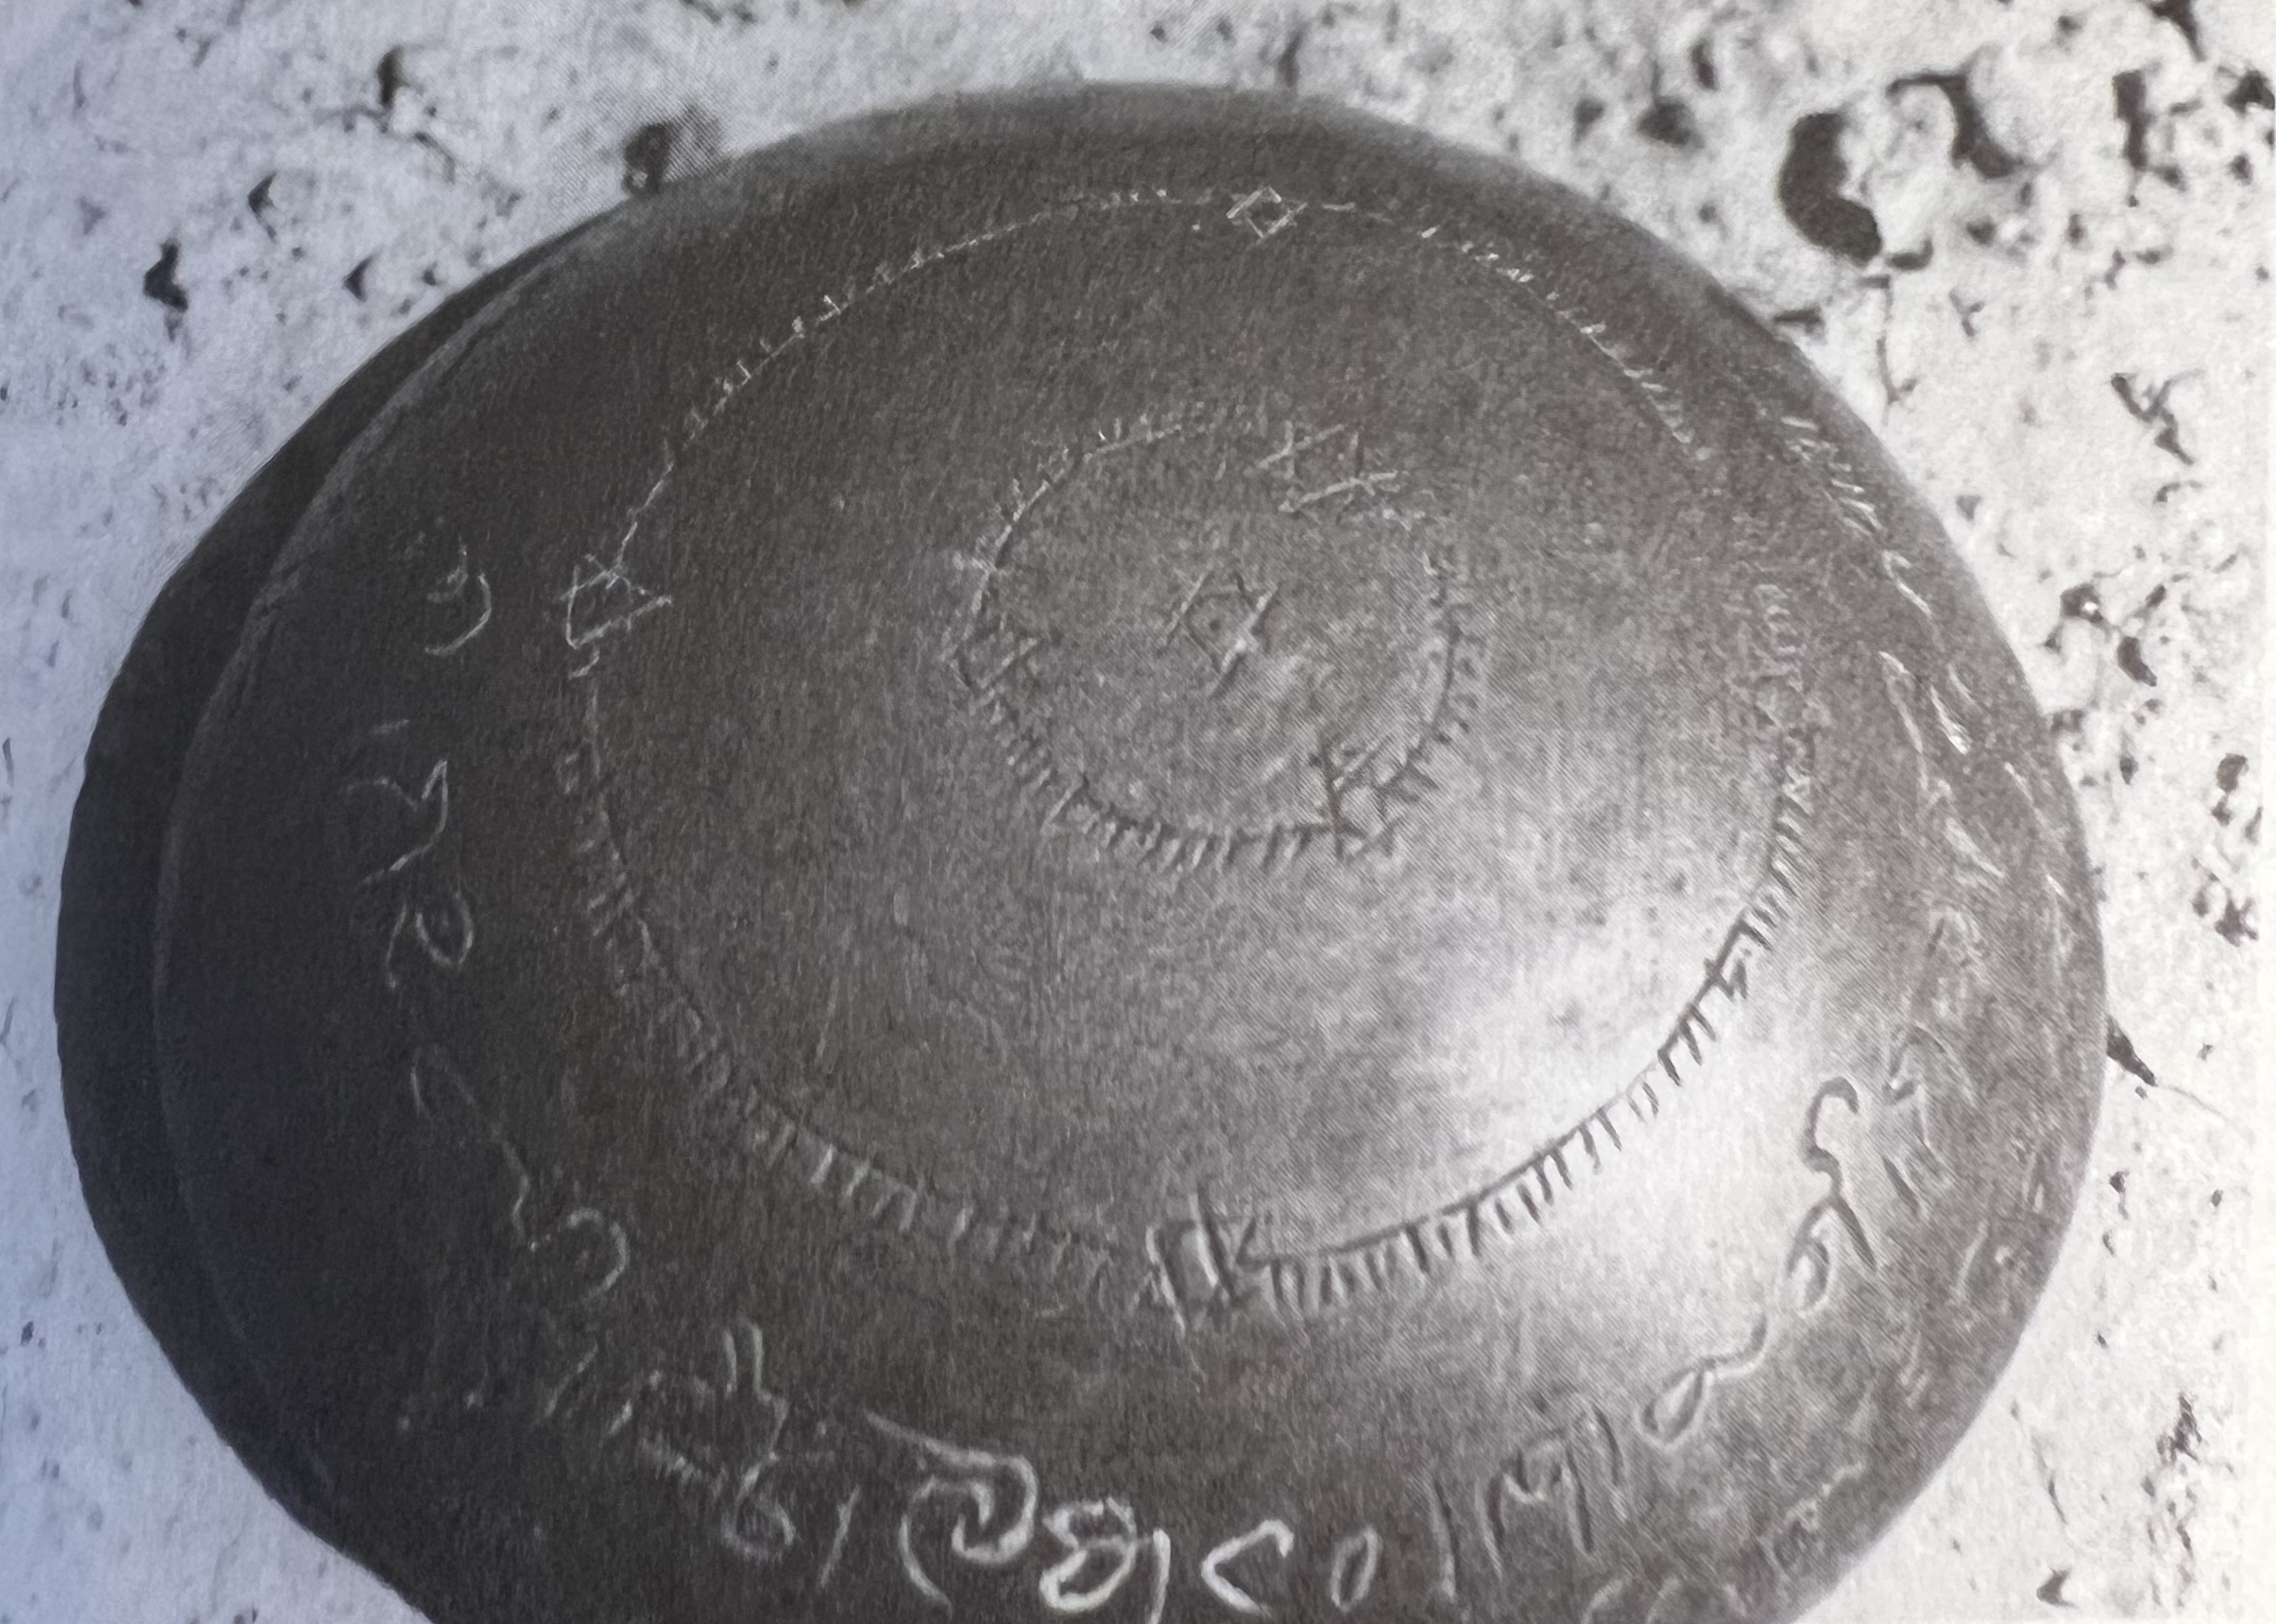
\includegraphics[width=\textwidth]{HommeetIslam/Images/IMG_2456recadre.png}
     \label{fig:my_label}
 \end{figure}

\paragraph{sceaux de salomon sur la paroi extérieure}La paroi extérieure comporte trois zones concentriques. Le fond de la coupe est occupé par un sceau de Salomon. Un premier anneau sur lequel s'alignent des bâtonnets est interrompu trois fois par des sceaux de Salomon, disposés en triangle. Un second anneau, situé dans la partie basse de la coupe, reprend le même système de bâtonnets et de sceaux, cette fois au nombre de quatre et disposés en carré. On dénombre ainsi huit sceaux de Salomon. Enfin, entre cet anneau et la lèvre, on relèvera deux lignes de texte. L'une, dont l'incision est plus profonde, se trouve gravée à proximité de la lèvre et s'étend sur tout le pourtour; elle indique :
 \begin{quote}
     « Hädhihi (2)\mn{Soit : « Celle-ci [i. e. cette coupe] [sert] pour la piga-re du serpent et du scorpion, les chiens enragés, à faciliter l'accouche. ment, aux saignements de nez, [pour les douleurs à] l'estomac ... (?), les coliques …. (?), un sceau de Salomon ... (?) »} li-lasat al-hayya wa al-agrab wa al-kalib (sic) al-kalib wo
li-usr al-walad wa al-ruäf wa al-miada ... (?) al-qawlanj ... (?) un sceau de Salomon ... (?) ».
 \end{quote}
 \paragraph{Un rajout : des objets qui vivent}Deux traits verticaux avec une barre médiane séparent le début de la fin de la phrase. L'autre inscription, située entre celle-ci et le second anneau, est incisée plus profondément, le trait en est plus épais que la précédente. Cela suggère un rajout,
le texte le confirme : 
\begin{quote}
    « Waqafa \mn{[legs pieux du Häjj Husayn al-Hawa (?) à la mosquée, la protégée, en 1313/1895-96]} al-Hajj Husayn al-Hawâ (?) \textit{hâ}dhihi al-
tâsa (sic) alâ al-Jâmi al-mahrûs 1313 »
\end{quote}   La lecture du nom du donateur pose problème, car un \textit{alif} semble avoir été tracé à la suite du \textit{hâ}', puis un \textit{waw} gravé en partie sur le \textit{alif} et avec la marque d'un rattachement à une lettre qui le précèderait, mais qui n'est pas donnée; enfin de petites encoches semblent indiquer une volonté de raturer ce \textit{waw}.
Ensuite apparaît un signe ressemblant à deux \textit{waw}-s inversés dont les boucles s'entrelacent : il peut être identifié comme une marque de fin de phrase, à la manière des petits décors que l'on trouve dans les manuscrits.

\subsection{la coupe B}
\paragraph{coupe B plus grande et ouvragée dans un alliage cuivreux}
La seconde coupe B, plus grande et plus ouvragée sur ses parois internes et externes au décor incisé, sans pied, à lèvre arrondie, a été réalisée dans un alliage cuivreux, et son fond, fendillé de manière semi-circulaire par l'usage, a fait l'objet d'une \textbf{réparation}. Il s'agit vraisemblablement d'une soudure. Ses dimensions sont de 6,5 à 6,6 cm de hauteur et de 18,3 cm de diamètre, mesuré de bord à bord extérieurs, la lèvre comptant pour 0,4 cm. Elle est de provenance inconnue. 

\paragraph{proche d'autres coupes se référant à Saladin}En ce qui concerne le décor de ses parois extérieure et intérieure, elle se rapproche d'autres coupes se référant à Abû al-Muzaffar Yûsuf (habituellement identifié comme Saladin), avec la liste de ses vertus curatives - il en sera question plus bas - mais s'en distingue, par l'absence de représentation de la Kaba en son centre (intérieur) (Savage-Smith, 1997, 73). Elle se rapproche davantage de quatre autres coupes, trois décrites par Rehatsek, et la quatrième, propriété du Science Museum à Londres. Elle n'est pas datée, mais à coup sûr fabriquée postérieurement à l'époque de Saladin,  semblablement entre le VIII-IX'/XIV°-XV° s. et le XII/XVIII, peut-être XIII /XIX s..
\begin{figure}
    \centering
       \sidecaption{Coupe B paroi interne}
 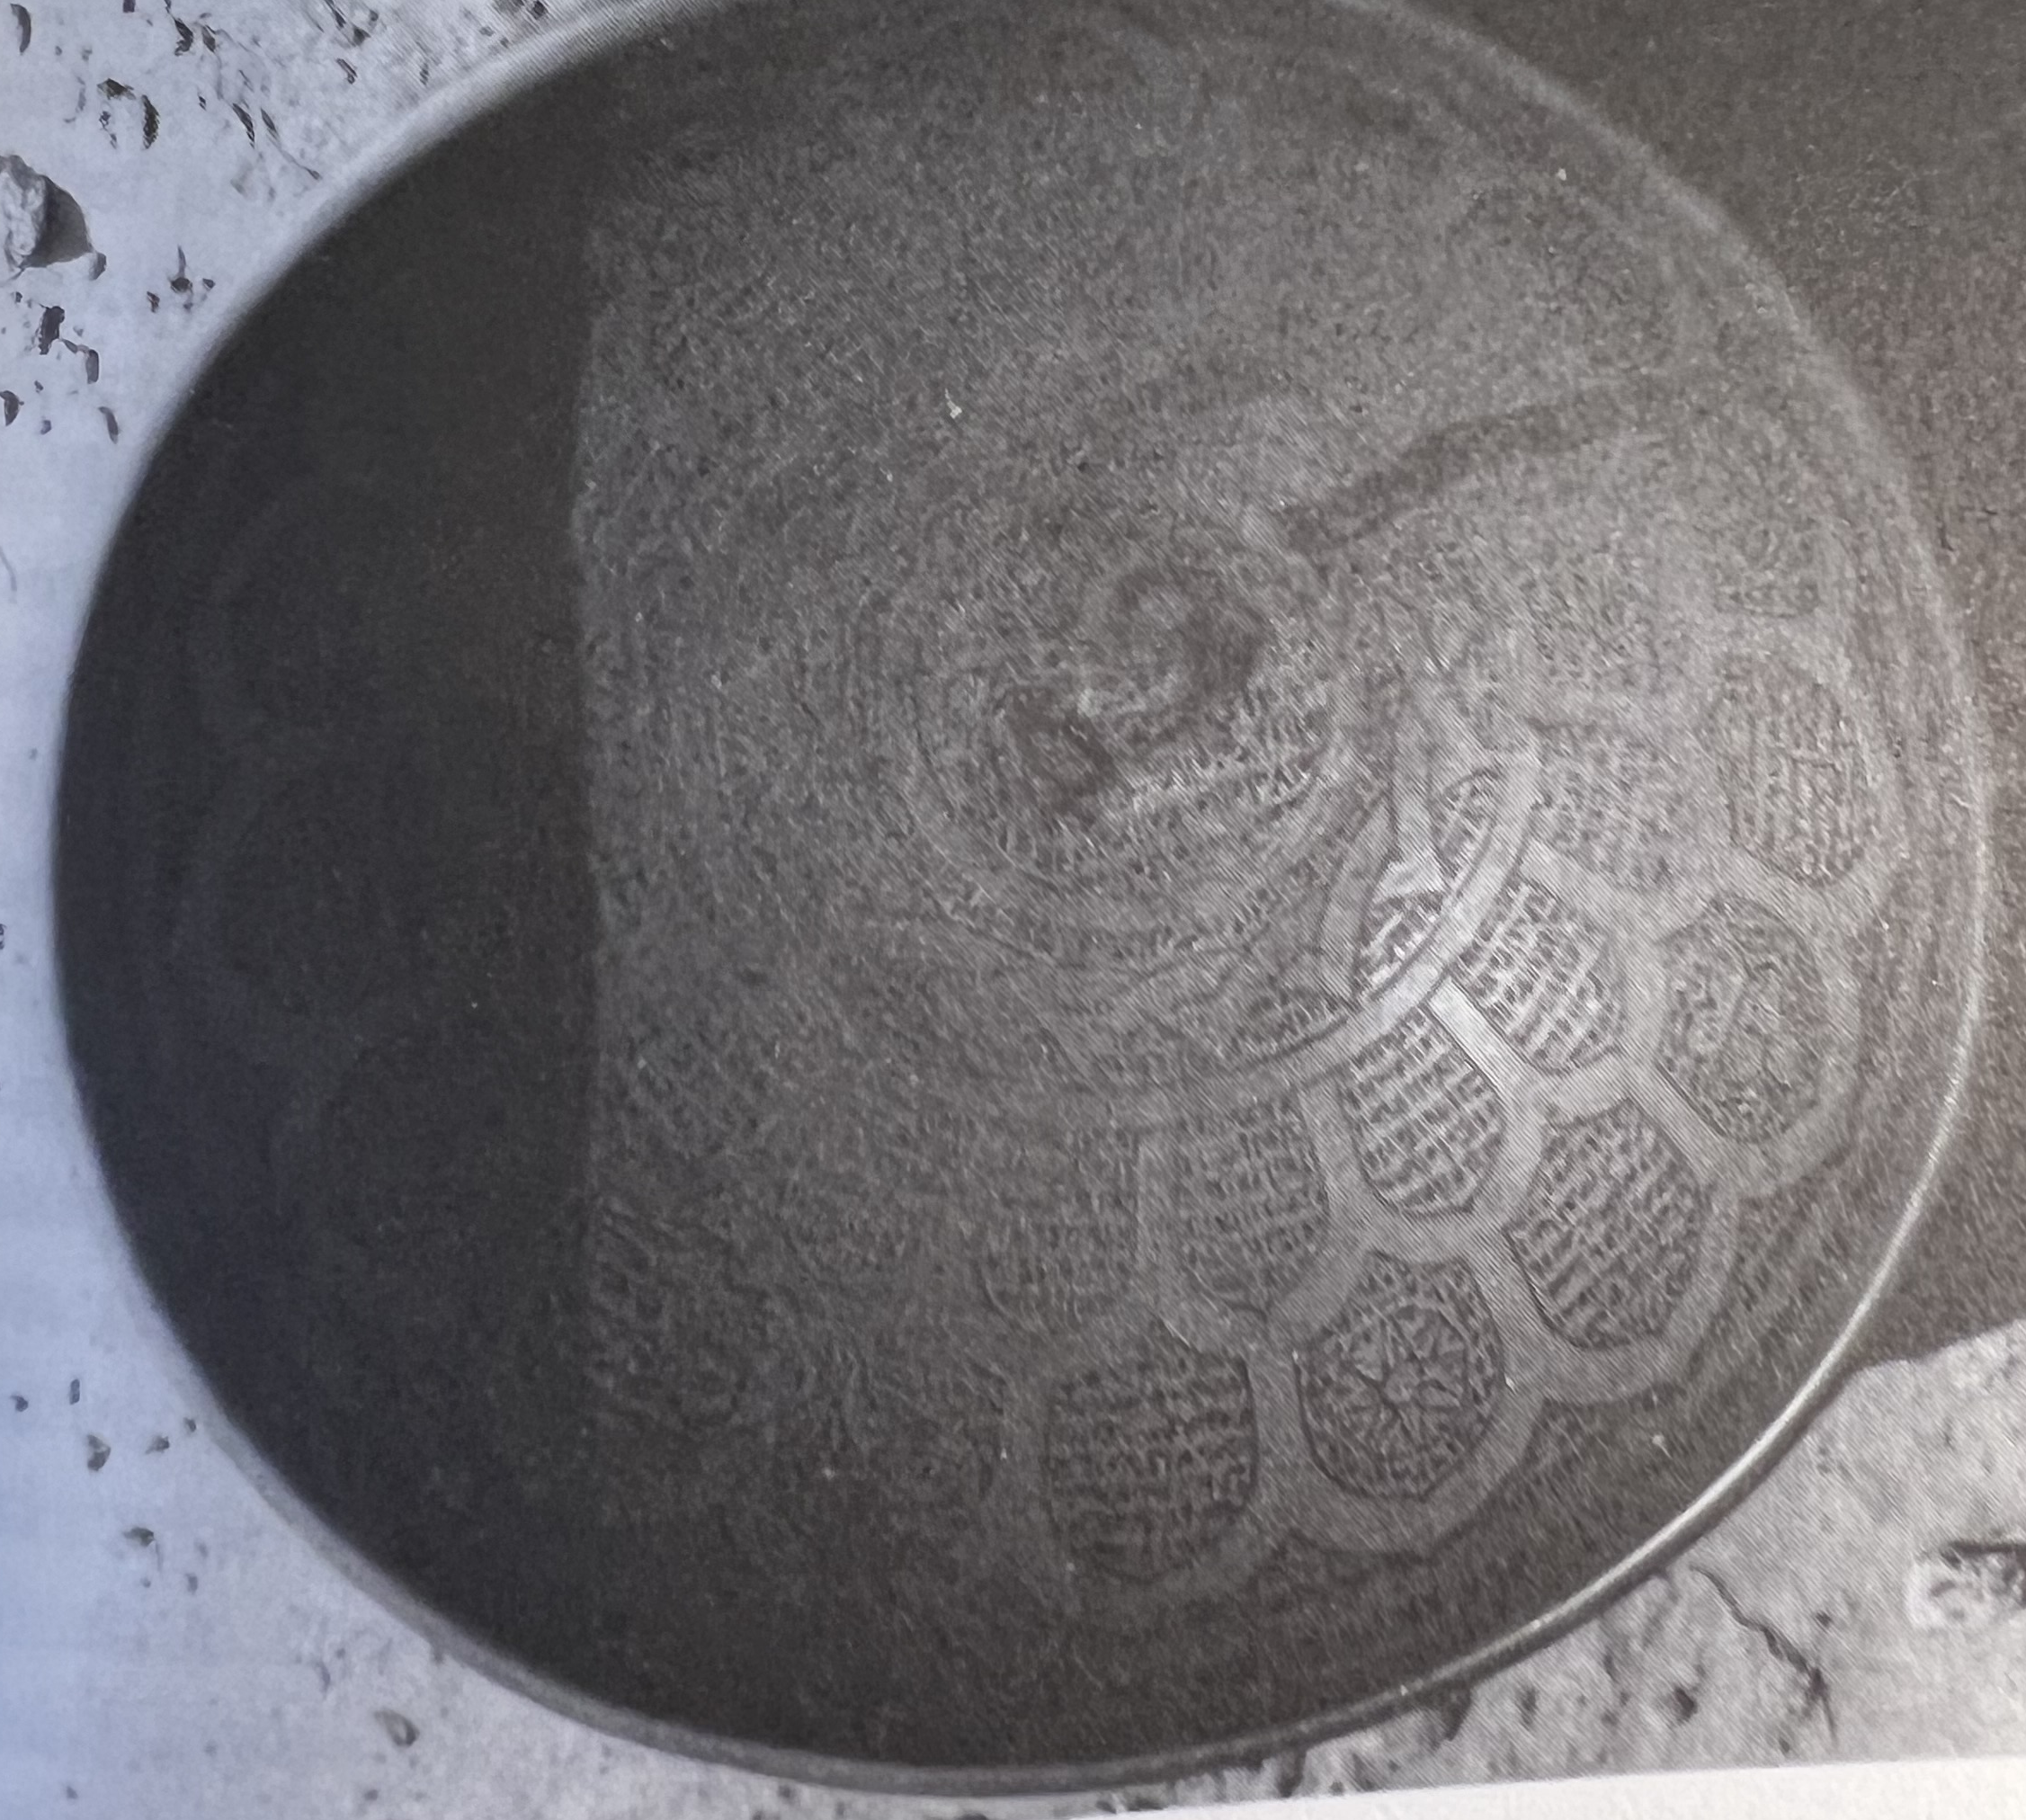
\includegraphics[width=0.8\textwidth]{HommeetIslam/Images/IMG_2457recadre.png}

 
    \label{fig:my_label}
\end{figure}

 \paragraph{3 registres concentriques}
L'ensemble du décor de la paroi intérieure se répartit sur trois registres, chacun délimité par un double cercle. On a ainsi trois doubles cercles concentriques dont le dernier suit les contours de la lèvre. 
Le premier registre, constitué par le fond de la coupe et délimité par un premier cercle concentrique, est occupé par un écrit de type magique qui reste à décrypter. On distingue autant que la détérioration et la réparation le permettent, des traits de hauteur inégale, des lettres de l'alphabet arabe. isolées, essentiellement \textit{hâ}', la (?), \textit{hâ} et \textit{kâf}, des chiffres, 6, 7, 95. Ils forment neuf lignes horizontales, la dixième suivant la courbure du cercle. Le second registre, situé dans la partie basse de la coupe, a essentiellement pour décor des bandes qui se chevauchent, formant seize pointes, une étoile à seize branches. L'espace résiduel est rempli d'écrits magiques, identiques aux précédents. Certains sont disposés sur le premier double cercle concentrique. Le troisième registre, enfin, occupe la plus grande surface de la coupe. Son décor est structuré par un motif de feuilles ou de pétales s'ouvrant en corolle, répartis sur deux hauteurs et décalés les uns par rapport aux autres. Ces « feuilles » forment autant de médaillons. La première série de médaillons, au nombre de seize, installée sur le second cercle concentrique, comprend exclusivement des écrits magiques identiques aux premiers, gravés sur six lignes, dont l'une est constituée par le second cercle concentrique. Quant à la série supérieure de seize médaillons, elle comporte, alternés, des représentations et des restes en arabe. 
\paragraph{un soleil, un chien, un scorpion, ...}On parvient à identifier les figures suivantes, dans le sens des aiguilles d'une montre : un soleil à huit rayons enfermé dans un cercle, un chien, un scorpion, un personnage (une femme avec un enfant, allaitant ?), un croissant de lune, un cheval, un serpent, un second personnage (personne mordue par un serpent ? ou possédée par un esprit malin ?). Autour d'eux, les mêmes écrits magiques, qui diffèrent cependant des précédents en ce qu'ils ne sont pas gravés sur des lignes.
L'ouvrage est fait de telle façon que la lune se trouve opposée au soleil, que l'un des personnages est dans l'axe de l'autre et les deux quadrupèdes face à face. En ce qui concerne les textes en arabe, il s'agit d'extraits du Coran, tous écrits sur huit lignes. En partant de la sourate liminaire, placée entre le chien et le scorpion, et en allant dans le sens des aiguilles d'une montre, on déchiffre :
\begin{enumerate}
   \item al-Fâtiha, jusqu'à
" .. ghayr al-maghdûb 'alayhim" ;
  \item précédée de la basmala,  une partie de s25v45 (« la Loi ou la
Salvation », al-Furqân), jusqu'à "la-jaalahu sâkinan", enchaînée à s6v13
(« Les troupeaux », al-An'âm), enfin quelques 4 mots non déchiffrés;
  \item la basmala, puis s84v1-4 (« La Déchirure », al-Inshiqâq), le verset
4 s'achève à : "wa algat má fiha", la fin reste à déchiffrer ;
  \item sans basmala, s24v35 (« La Lumière », al-Nür), jusqu'à « Júgad
min shajara mubâraka zaytâna là sharqiyya wa là [gharbiyya] », quelques lettres isolées (?), puis ra', les chiffres 7 et 2 ou 3
  \item la basmala, puis sur la 2° ligne, les 3 lettres liminaires apparaissant
au début de six sourates, celles de la Vache, d'al-'Imran, de l'Araignte, des Romains, de Lugmân et de la Prosternation (soit 2, 3, 29, 30, 31 er
32), à savoir \textit{alif}-lâm-mim, suivies de 3 mots non déchiffrés, puis sur la 3ème ligne, les 5 lettres liminaires de s19 (« Marie », Maryam), à savoir \textit{kâf}.
hã'-ya'-ayn-sâd, suivies de quelques mots non déchiffrés, puis sur la 4. ligne, les 3 lettres liminaires du début de s26 et   28 (« Les poètes » et « le
récit », al-Shu'ara' et al-Qasas), à savoir tâ'-sîn-mim, enfin les autres
lignes n'ont pu être déchiffrées ;
  \item la basmala, suivie de deux lignes et demi non déchiffrées, puis viennent peut-être une partie de s16v69 (« Les Abeilles », al-Nahl),
« yakhruj min butûni\textit{hâ} sharâb mukht\textit{alif} alwânuhu fihi shif@' » (?), et une partie de s17v82 (« Le Voyage nocturne », al-Isrâ'), « wa-nunazzil
min al-Our'ân mâ huwa shifà »" (?) ;
  \item la basmala (?), puis on lit \textit{hâ}-\textit{alif}, lâm-\textit{hâ}' al-rahmân al-rahim), suivi de s8v62-64 (« Le Butin », al-Anf@l) : le dernier mot du v63,
« hakîm », n'est pas très lisible et le v. 64 est déchiffrable jusqu'à « hasbuka Alla », quelques mots restent ensuite à comprendre;
  \item) sans basmala, 2v255 (« La Vache », al-Bagara, « verset du
Trône », ayat al-kursi), jusqu'à : « ... là yuhîtûn »'.
\end{enumerate}

L'espace compris entre les médaillons et l'ultime double cercle est
occupé par les écrits magiques déjà rencontrés plusieurs fois. Sur le cercle supérieur de ce dernier double cercle, enfin, est gravée une rangée
des mêmes écrits. Le décor de la paroi extérieure offre trois registres. Le premier est constitué par le fond de la coupe qui laisse deviner, en dépit de l'usure, le même type de composition magique que sur la paroi intérieure; la forme géométrique qui l'enserrait a disparu. On reconnaît ensuite un cercle concentrique constitué encore des écrits magiques. Le second registre occupe la partie médiane de la coupe. Les écrits magiques sont cette fois inscrits dans cinq cercles et cinq trapèzes alternés. Enfin, le troisième registre présente une ligne d'écriture qui suit le bord de la lèvre et s'étend sur tout le pourtour. Elle est gravée de telle sorte que le début du texte s'enchaîne sans rupture avec la fin. Cette phrase ininterrompue pourrait tenir dans un double cercle concentrique : le graveur s'est appliqué à ne jamais en dépasser les limites invisibles et à emplir l'espace de telle sorte qu'elle donne l'impression d'une bande circulaire continue, très décorative. Elle est chargée d'indiquer les vertus curatives de la coupe, comme c'est le cas pour la coupe A:
\begin{quote}
    « wa  li-mawlâna al-sultân al-Malik al-Mujähid al-muwakkal al-man.
sûr Abû al-Muzaffar Yasuf wa jumi a fiha manâfi mujarraba wa hiya li-
las'at al-hayya wa al-'agrab wa-li-al-hummâ wa al-mutlaga wa al-magh-
la wa li-al-kalb al-kalib wa li-al-maghass wa al-qawlanj wa al-shagiga
wa al-zarabân (?, sic) li-ibtâl al-sihr wa li-ramì al-dam wa li-al-ayn wa
al-nazra wa li-râd al-lawaga wa li-ifâdat al-masrû (?) wa li-usr al-baw!
wa li-sulh bayn al-aqrân (al-agrâb ?) wa li-nakad al-atfäl wa al- m.r: (?.
ou 'm.r.j?) bi\textit{hâ} al-mashür wa al-musâb wa al-bint (?) al-mu sira" ».
\end{quote}
Soit :
\begin{quote}
    {  « Pour notre Seigneur, le Sultan, al-Malik al-Mujähid, le manda-victorieux Abû al-Muzaffar Yûsuf26. Y [la coupe] sont réunis des bienfaits éprouvés par l'expérience, elle [sert] pour les piqûres de serpent et de scorpion, pour la fièvre, la parturiente? et augmenter le lait, pour les morsures de] chiens atteints de la rage, pour les douleurs stomacales et les coliques, la migraine et les élancements (?)?, pour conjurer les sortilèges, ou faire cesser le flux du sang, pour le mauvais œil et le mauvais sort  
pour empêcher la paralysie faciale et pour le rétablissement de la conscience des épileptiques (?), pour la dysurie, pour la réconciliation des adversaires (ou : les proches parents ?), pour les enfants agités. L'ensorcelé et celui qui est atteint, de même que la parturiente en difficulté (?), doivent [en boire le contenu par gorgées (?)].}
\end{quote}
\paragraph{Titulature de Saladin mais pseudo-épigraphique}
La titulature, la \textit{kunya} (= Abû al-Muzaffar) et le nom (ism = Yûsuf) \sn{à
moins qu'il ne s'agisse que d'une kunya = Abû al-Muzaffar Yüsuf}, mentionnés dans l'inscription, peuvent-ils servir à identifier le personnage ?

Et constituent-ils un élément fiable de datation de notre objet ? La même formule (sauf al-muwakkal) se retrouve chez Reinaud, sur les coupes n° 9420, chez Wiet, n° 14, chez Canaan - qui n'identifie pas - et surtout sur les deux coupes, dites de Saladin, étudiées par Zéki Pacha : \begin{quote}
     Izz li-mawlâna al-sultân al-malik al-mujâhid al-muayyid al-Mansûr Abû al-Muzaffar Yûsuf » et : « 'Izz. li-mawlânâ al-sultân al-malik al-mujâhid Abû al-Muzaffar Yasuf »
\end{quote} Les coupes dédiées à Saladin sont réputées nombreuses   mais ne sont pas nécessairement indicatrices d'un temps et d'un lieu de facture particulier. 
En effet, Wiet (1922, 319-28), dans un article très précis, critique la datation de Zéki Pacha en s'appuyant essentiellement sur des documents épigraphiques, mais aussi sur des chroniques : il montre que les inscriptions de ces deux coupes font entorse à la titulature de Saladin, et donc au protocole habituel, que ces formules sont rares au VI/XI s., et que les dates qui suivent la mention de souverains, sur les coupes, ne sont pas un gage de leur époque de fabrication; il concède toutefois que l'on puisse y voir une allusion au souverain ayyûbide - si l'on se rapporte à d'autres objets sur lesquels se trouve le même type d'anomalies - mais qu'en aucun cas, ces coupes ne peuvent être contemporaines de Saladin. Le style de la coupe B, de même que les conclusions de Wiet, font plutôt penser à une attribution posthume.
\begin{figure}
    \centering
       \sidecaption{Coupe B paroi externe}

  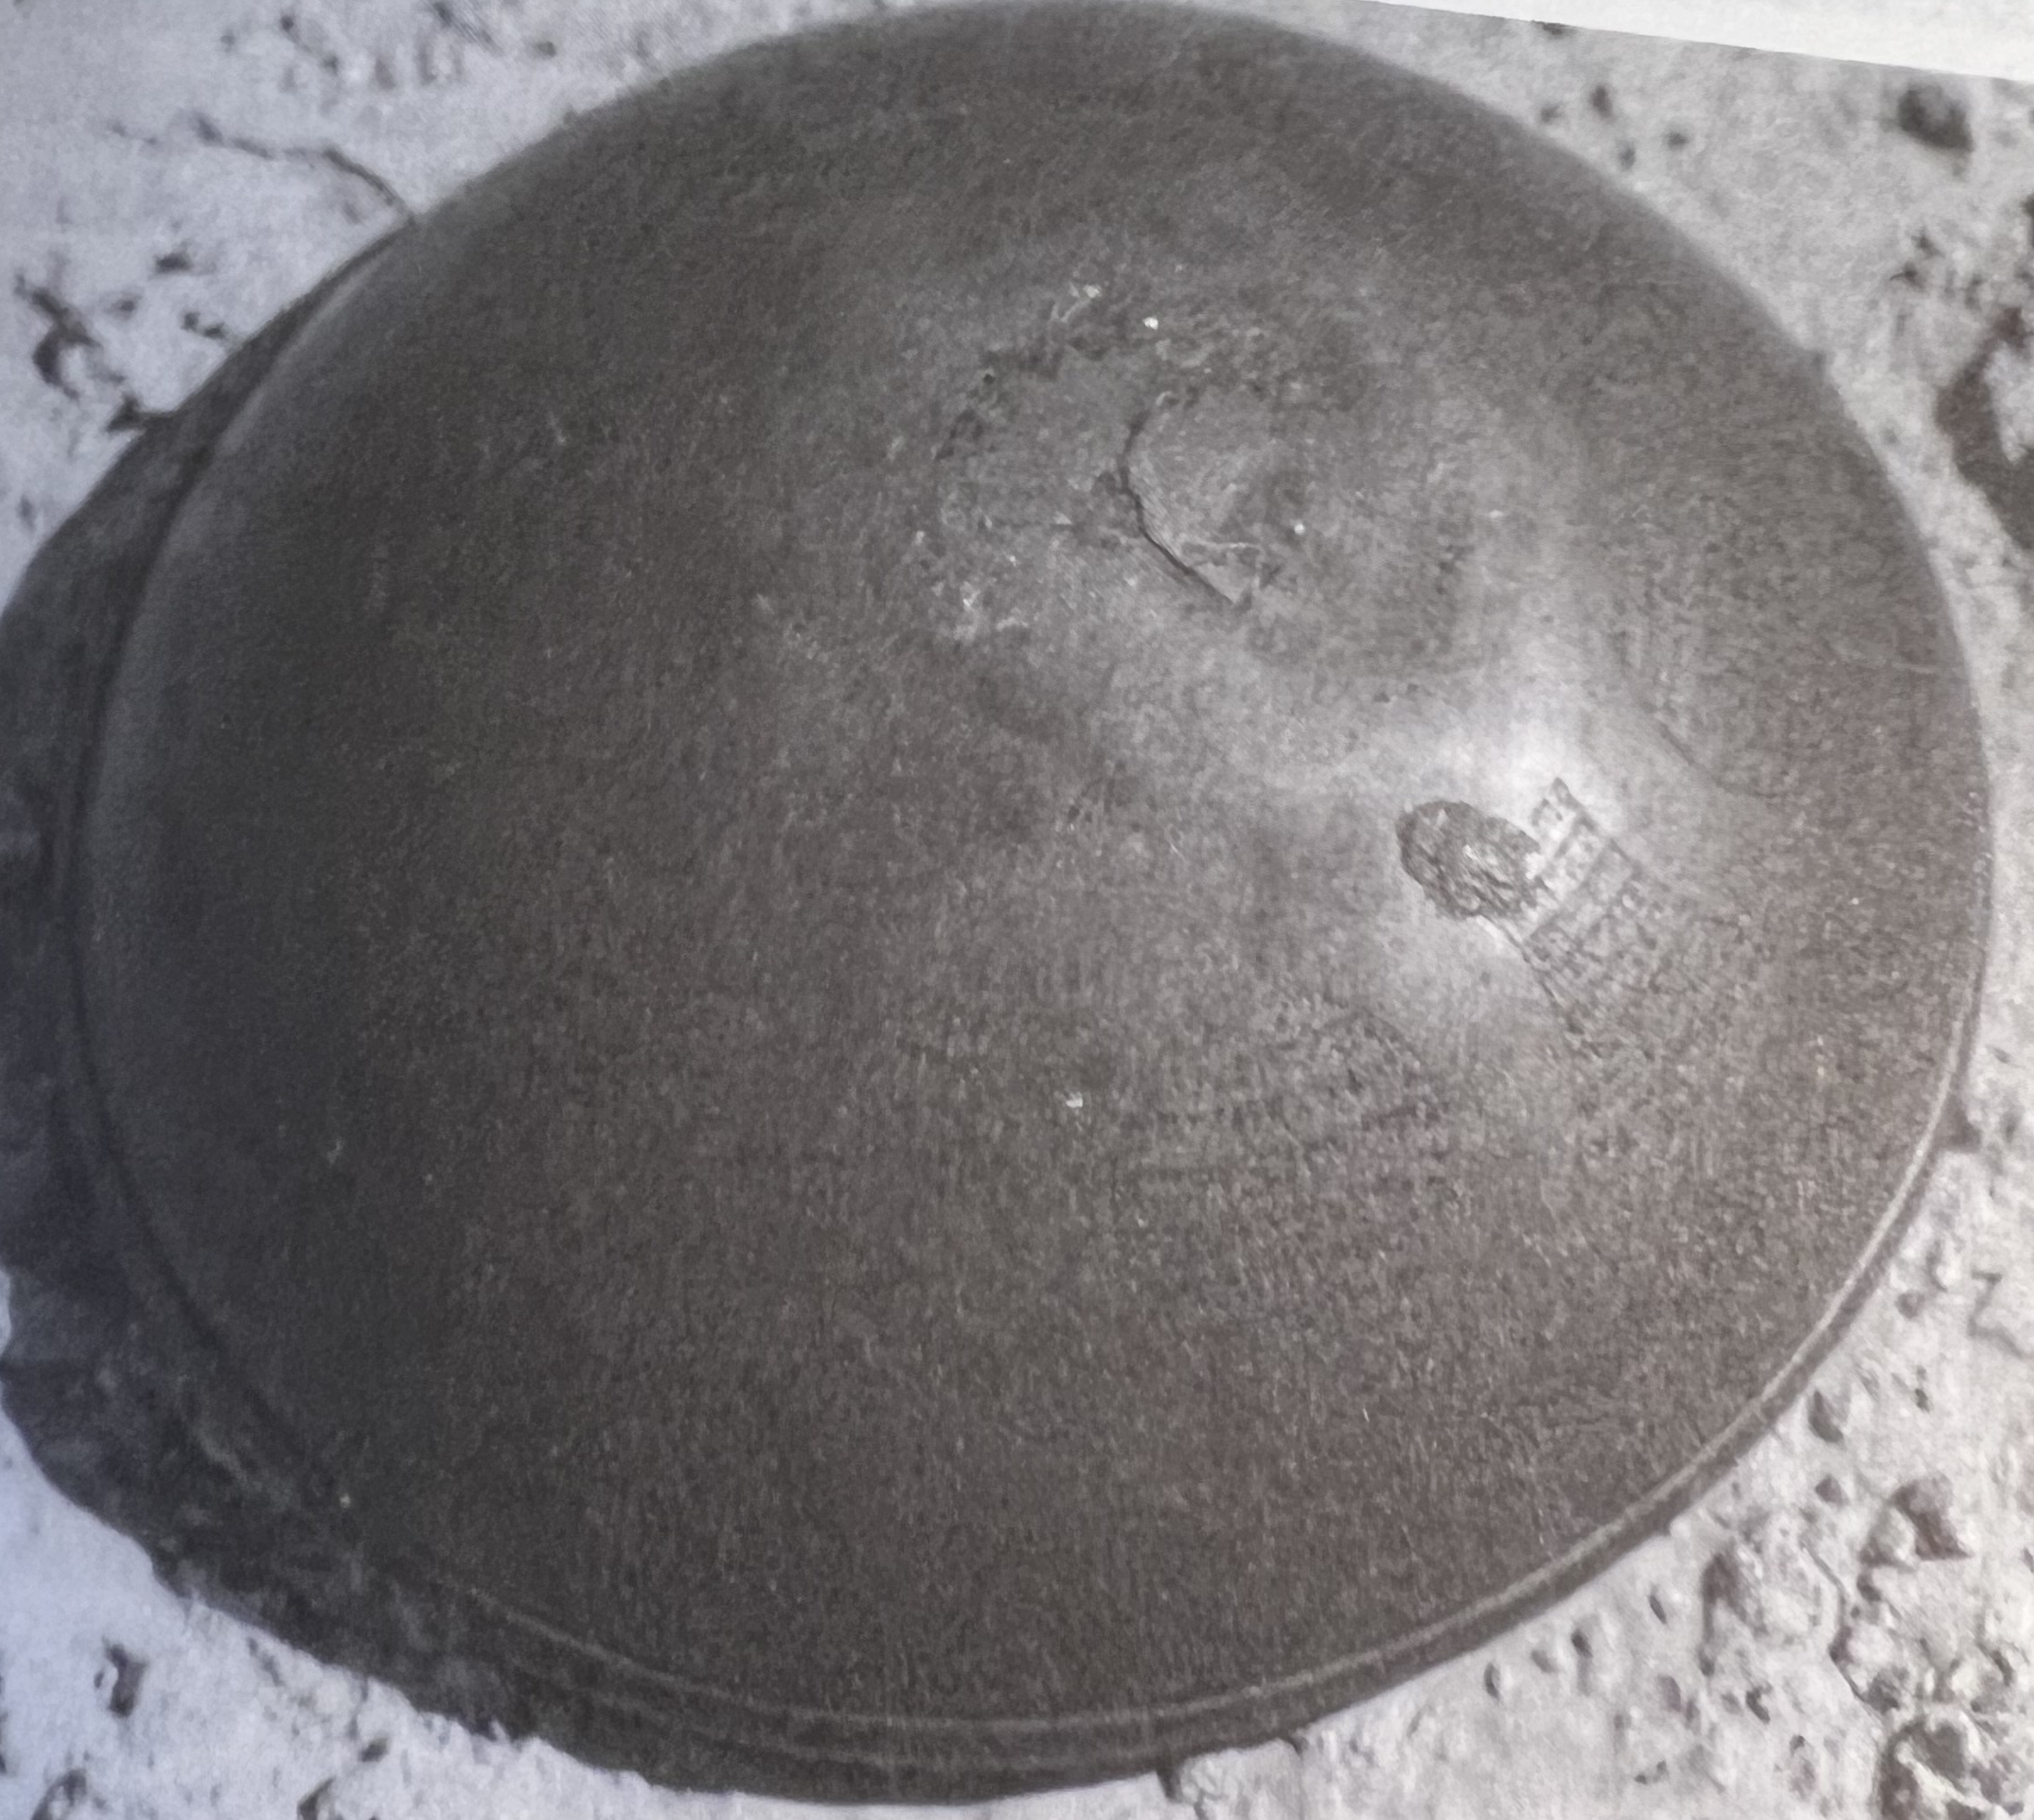
\includegraphics[width=\textwidth]{HommeetIslam/Images/IMG_2458recadre.png}

 
    \label{fig:my_label}
\end{figure}
  \paragraph{coupe anti poison}
L'étude des écrits, représentations, signes et figures géométriques des deux coupes fait apparaître un registre commun avec la talismanique. La symbolique de la coupe A, telle qu'elle se dégage à partir des éléments décrits, vient confirmer certaines de ses propriétés curatives. Tout d'abord, il s'agit d'une coupe anti-poison ; 

\paragraph{incantation valable pour toute oeuvre magique tenant compte de l'Evangile et de la Torah}al-Bânì cite une longue incantation (\textit{azima}) versifiée, valable pour toute œuvre magique : elle décrit les sept lettres spéciales, rappelle qu'elles sont le nom suprême de Dieu, puis que moyennant l'ajout de lettres de la Torah, des Evangiles et du Coran, l'on sera protégé des serpents, scorpions et lions?. Il s'agirait donc, dans l'ensemble, des animaux nuisibles ou devenus dangereux dont la coupe guérit de la morsure ou de la piqûre. En outre, elle aide en cas d'accouchement difficile, ce qu'indique la présence de la sourate \textit{al-
Inshiqâq}. 

\paragraph{coupe d'accouchement; analogie terre et accouchement  }
Des textes gravés sur d'autres coupes comparent le mouvement de la terre qui rejette ce qui est en elle et se vide, à celui de la femme qui met un enfant au monde dans des conditions favorables. Spontanément, les deux coupes m'ont d'ailleurs été présentées comme des « coupes pour l'accouchement », l'usage ayant probablement consacré cette fonction entre toutes. Selon al-Bûnî (s.d., (a), 91) encore, les trois bâtonnets, sans l'\textit{alif} sur le dessus, désigné simplement alors comme « protubérance » ou pointe de lance, et accompagnés du pentagramme, peuvent être employés pour guérir des maladies affectant l'intérieur du corps, dont les coliques (\textit{gawlanj}), auxquelles fait référence la liste des maux soignés par la coupe A. 
\paragraph{sceau de Salomon, sur les rouleaux Ethiopiens}
Enfin, les deux carrés entrecroisés gravés à l'intérieur de la coupe forment une étoile à 8 branches - cette étoile finissant dans un double cercle peut aussi représenter le soleil, dardant ses rayons? -. Décrite comme la gravure ou le diamant de l'anneau de Salomon, l'une de ses variantes se trouve sur les rouleaux magiques d'Ethiopie, où elle est appelée « sceau de Salomon »». Son centre, qui est également le centre de la paroi interne, est entièrement occupé de bâtonnets magiques. 
\paragraph{Pouvoir du roi Salomon - de son sceau}
Qu'il soit bague ou talisman, selon la Tradition, il donne à ce Roi son pouvoir sur les démons
-  pouvoir que le Coran lui reconnaît, dans la sourate Sâd, aux versets 34-39 - et donc sur la cause des maladies, ou tout au moins de certaines.
Dans certaines versions, il oblige les démons, qui sont des sortes de gardiens des maladies, à livrer les remèdes (Barkaï, 1996, 193). Dans l'ensemble, les démons - parfois appelés djinns - sont divisés en tribus liés à un habitat, et la maladie est ainsi territorialisée. Salomon n'éradique certes pas la maladie, mais, grâce à la puissance de son sceau, don du ciel, il est celui par lequel vient la guérison. On remarquera que le sceau de Salomon est gravé ici parmi les maux que la coupe est censée soigner.

\paragraph{Principe de guérison}
Leur liste étant incomplète, on ne fera qu'évoquer les maladies spécifiquement provoquées par les djinns ou les démons que Salomon et ses formules peuvent exorciser. Pour ce faire, on doit s'asperger ou se laver avec l'eau versée dans la coupe. L'architecture de la paroi interne est ici toute conçue et rythmée à partir de ce motif. Elle est largement construite selon le chiffre huit ou ses diviseurs. L'étoile à huit branches et les huit étoiles à six branches, structurant les parois interne et externe, indiquent singulièrement qu'elle en appelle à la protection de Salomon par qui vient la guérison, les autres grands pourvoyeurs de guérison étant Dieu et le Prophète (évoqué dans la formule gravée près de la lèvre supérieure de la coupe A).


La coupe B présente également l'image des animaux à piqûre et morsure (scorpion, serpent, chien, cheval) et le début de la \textit{sourate de la Déchirure}. L'un des deux personnages (femme avec un enfant, l'allaitant ?) rappelle son pouvoir de faire venir le lait. La \textit{basmala}, prononcée avant toute action et notamment avant d'ouvrir la bouche pour manger, de même que les Versets du Siège, appelés \textit{âyat al-hars wa l-hirz}, protègent contre les mauvais dinns ou démons. C'est le cas également des cercles.

\paragraph{sourate pour chaque maladie}
Thème que pourrait reprendre encore l'un des deux personnages (personne possédée par un esprit malin ?). Deux sourates renvoient aux sources de la guérison plutôt qu'elles ne visent une maladie en particulier. Le verset 69 de la sourate des \textit{Abeilles} fait en effet allusion aux pouvoirs curatifs du miel, qui fait partie des liquides versés dans les coupes, selon mon informateur, et à absorber donc par les malades. Les vertus du miel sont extrêmement nombreuses et constituent un thème de prédilection de la médecine prophétique. Par ailleurs, s17v82 (« Le Voyage nocturne ») rappelle le pouvoir curatif du Coran. D'une manière plus générale, s8v62-64 (« Le Butin ») martèle l'idée que : \textit{« Dieu te suffit »}. Quant à la sourate liminaire, ses vertus sont tellement innombrables, qu'elle n'est plus indicative : elle est bonne pour tout. Enfin, les deux Luminaires, le soleil et la lune, sont des symboles de vie, de prospérité et d'abondance, comme le remarque Canaan (1936, 100, 121). De la même manière que les deux Carrés entrecroisés contenant des écritures magiques, à l'intérieur de la
 coupe A, peuvent représenter le soleil sous la forme d'une étoile à huit pointes et qu'elle est structurée selon le chiffre huit, le soleil, dans la coupe B, compte également huit pointes. Par ailleurs, le fond de la coupe B est occupé par une étoile à seize branches, qui soutient sa composition interne en seize médaillons, puis en deux fois huit médaillons (à texte et à figures). Quelques coupes étudiées par ailleurs montrent une corrélation entre la présence des Luminaires et le chiffre 16 (cartouches ou cercles).
 \paragraph{Chiffre 8 et soleil}
Le rapport est donc net entre le chiffre huit et le soleil. On est tenté de mentionner alors le fait que huit correspond à la valeur isopséphique du \textit{hâ}, lui-même clé de la vie (hayât), selon un procédé bien connu en science des lettres. Cependant, les versets des sourates 6, 24 et 25, gravés sur la coupe B, rappellent l'omnipotence et l'omniscience de Dieu, cause de tout et à qui tout doit revenir, au-delà des deux Luminaires : 
\begin{quote}
   « C'est à lui qu'appartient ce qui subsiste dans la nuit et le jour »; « Dieu est la lumière des cieux et de la terre ».

\end{quote}
En guise de remarque finale sur les deux coupes, ne peut-on pas dire qu'elles contiennent ce qu'appartient ce qui subsiste dans la nuit et le jour ; \begin{quote}
    « Dieu est la lumière des cieux et de la terre ». 
\end{quote}
\paragraph{Cosmos}
En guise de remarque finale sur les deux coupes, ne peut-on pas dire qu'elles constituent une tentative de reproduire le monde clos du cosmos ?
\begin{figure}
    \centering
        \sidecaption{La Coupe comme représentation du cosmos. Coupe B paroi Interne et externe}
\includegraphics[width=\textwidth]{HommeetIslam/Images/IMG_2459recadre.png}

    \label{fig:my_label}
\end{figure}




En effet, le soleil qui préside à l'architecture interne des deux coupes, les cercles concentriques, les entrelacs de rubans ininterrompus, les textes eux-mêmes parfois écrits de telle manière qu'ils ne s'achèvent ni ne commencent, les motifs alternés qui se répondent, ainsi que la concavité et le caractère hémisphérique des deux objets (Canaan, 1936, 82), sans compter la composition organisée en registres, concourent à le reconstituer, quelques sourates rappelant que Dieu demeure le plus puissant, le plus savant et la Cause unique et suprême. Si l'on songe que le mode d'emploi des coupes consiste à passer par un liquide qu'on y verse, celui-ci se trouve donc en contact avec toute chose du monde : ambition holistique des coupes.
\paragraph{contexte Yemenite en cas d'accouchements et poisons}
Le recours aux coupes thérapeutiques est d'un usage bien établi au
Yémen, aussi bien dans la communauté juive que musulmane (Brauer, 1934, 182-3), surtout dans les cas d'accouchements difficiles ainsi que, concurremment à d'autres pratiques, contre le venin des serpents. L'acte de soigner différents venins, parmi lesquels celui des scorpions, est particulièrement investi par diverses médecines ou pratiques. C'est sans doute un indice de la fréquence du danger. 
\paragraph{fonctionnement des coupes : boire}
Selon l'un de ceux qui ont la responsabilité des coupes à la mosquée, leur mode d'emploi consiste principalement à boire le liquide - de l'eau, du bouillon - ou le miel que l'on y a versé. Le docteur Sarnelli rapporte, pour le Yémen des années 30, qu'il faut boire l'eau à petites gorgées en prononçant des louanges à l'endroit lu Seigneur des mondes, de ses anges et de ses prophètes. Pour les mêmes années, Brauer cite d'autres manières de les utiliser chez les juifs yéménites, il en sera question un peu plus loin (Brauer, 1934,182-3). Une véritable description ethnographique, susceptible de nous renseigner sur ensemble des étapes à suivre pour utiliser les coupes, manque cependant, que ce soit pour le Yémen, ou un autre lieu.
\paragraph{hypothèse : produit au contact des écrits communique au patient}
Le produit en contact avec l'ensemble des écrits et l'iconographie est chargé de communiquer quelque chose au malade, mais selon un principe qui reste à définir. Le liquide en relation avec les représentations des animaux nuisibles transmet-il au patient une partie de leur force, l'immunisant par assimilation de quelque chose de leur substance, agissant tel un contrepoison ? Ou au contraire, s'agit-il d'une mithridatisation\sn{Le fait de mithridatiser, d'immuniser en accoutumant à un poison.} ? Les présentations ont-elles une valeur prophylactique\sn{Qui prévient la maladie.
Mesures d'hygiène prophylactiques.}, comme c'est le cas sur des talismans chassant les bestioles et les chiens des maisons (Doutté.
194, 144-46) 
\paragraph{seéquence écrit liquide boire}
  La séquence écrits-liquide-boire, enfin, rappelle une pratique présente dans l'ensemble du monde arabe, qui consiste à écrire in papier, à l'encre noire ou de couleur, généralement des versets coraniques, et à le tremper dans un récipient empli d'eau, que l'on demande au malade de boire, notamment dans les cas d'ensorcellement!.

  \paragraph{bouillon, pratique aidant les paturientes, mélange de pratiques médicales}
Cependant, dans le contexte yéménite des hauts plateaux, il semble que le bouillon versé dans les coupes serve à soutenir plus spécialement les femmes en couches. Le bouillon de viande (\textit{marag}) est gras, robotif, et rassemble la substantifique moelle de la viande : il est offert en début de repas et particulièrement aux hôtes, comme un met prisé et recherché, le meilleur en somme. Il est par conséquent indiqué pour soutenir physiquement la femme en travail. Ici, le liquide n'est donc pas seulement conducteur ou à la rigueur stimulateur, dans l'économie de la guérison par les coupes, mais il apporte ses vertus propres, qui viennent en addition de celles des écrits et représentations. En médecine domestique, pour la même région du Yémen, le recours simultané à des médecines et à des médications différentes est courant. Plutôt que le reflet d'un tâtonnement thérapeutique, il faut y voir au contraire un discernement et la volonté \textit{d'attaquer le mal, dans son éventuelle pluralité}, dans toutes ses facettes. Les symptômes sont en effet soigneusement observés et triés, et, à partir d'eux, il s'agit d'évaluer les causes, qui peuvent être diverses pour un même symptôme. Symptômes et causes ne peuvent être tous traités de la même manière, et entraînent la décision de recourir à tel ou tel praticien. 
\paragraph{la maladie comme résultat de causes multiples}
En outre, lorsqu'il y a maladie, elle est toujours soupçonnée d'être le résultat de causes multiples, de nature diverse, déchaînées en même temps. L'utilisation des coupes, dans le cas qui vient d'être évoqué, n'est clairement pas un acte médical unique.
Des traînées de bougie apparaissent au fond de la coupe B. Sont-elles en rapport avec l'utilisation des coupes ? Enfin, on observera que la coupe B, réparée, est toujours considérée comme en service. Pourtant, les détériorations et les réparations ont entraîné, pour partie, la disparition du décor gravé au fond. 
\subsection{Institutionnalisation de pratiques magiques} \mn{\href{https://books.openedition.org/ifpo/1264?lang=fr}{le waqf} Deux catégories de waqfs selon la nature de la nue-propriété du bien :
\textsc{Waqf ṣaḥîḥ}. constitué de biens-fonds issus d’une propriété privée (\textsc{milk}) appartenant au fondateur lui-même et uniquement à lui-même. Ce waqf est une fondation ṣaḥîḥ, véritable et intégrale 
 
    \textsc{Waqf ghayr ṣaḥîḥ} composé des biens mîrî.   propriété d’État, lequel a sur eux tous droits d’exploitation et d’imposition. Tous ces droits sont exercés sous la tutelle du waqf. 


Le terme « \textsc{bīmāristān} », ou « māristān »,  désigne un établissement hospitalier pour les malades dont on espère la guérison.
}
 
 

\paragraph{un bien waqf depuis 1895}
Que ces objets soient \textit{waqf} et non \textit{milk} ne fait aucun doute pour leurs gardiens. On trouve d'ailleurs gravé sur la paroi externe de la coupe A, à la suite de la liste de ses propriétés, l'indication suivante: 
\begin{quote}
    « Wagafa al-
Hajj Husayn al-Hawâ (?) \textit{hâ}dhihi al-tâsa (sic) 'alâ al-Jâmi al-mahrûs
1313 » [legs pieux (\textit{waqf}) du Häjj Husayn al-Hawa (?) à la mosquée, la protégée, en 1313/1895-96]. 
\end{quote}
Outre l'intérêt immense d'avoir ici une date, certes tardive et à ne pas prendre pour une date de fabrication, on retiendra qu'un tel statut pour un tel objet est bien un fait. Et le cas qui nous occupe n'est peut-être pas singulier. 

\paragraph{les outils des hôpitaux sont \textit{waqf}} L'une des coupes signalées par
Ahmed Zéki Pacha, provenant du Bimâristân al-Mansär - du nom de son
fondateur al-Malik al-Mansûr Qalâwûn, en 683/1284, au Caire - et encore en service à la fin du XIX s., permet sans doute de ne pas limiter
au Yémen zavdite. L'ensemble des instruments utilisés à l'hôpital était en effet considéré comme \textit{waqf}. 
\paragraph{waqf oral sans enregistrement pour les objets}
Cependant l'établissement du statut juridique des objets qui nous occupent, pose problème.
Tout d'abord, ils ne seraient pas recensés par le registre des \textit{waqf}s. Il est difficile de croire à une négligence d'autant que leur qualité de bien \textit{waqf} n'est pas dissimulée. En 1998, dans une ambiance peu favorable il est vrais, la tentative de consulter ces registres du Ministère des \textit{waqf}-s a tourné court. Mais aux alentours de 1999, les objets semblent avoir été récupérés par ce même Ministère, selon ce qu'a révélé une nouvelle visite au lieu où ils étaient auparavant déposés. Jusque là, ils semblaient échapper au contrôle de l'administration des \textit{waqf}-s et à toute redevance.
Ils m'ont été présentés comme « \textit{waqf}-s oraux ». La procédure paraît connue et rodée. Le donateur vient et dit au récipiendaire : \begin{quote}
    « Je donne cet
objet en \textit{waqf} à la mosquée [awgaftu \textit{hâ}dha al-shay' alâ Jâmi kad\textit{hâ} ».
\end{quote} 
Et voilà tout. Elle est adoptée pour des objets isolés, tels les corans, les tapis, offerts à la mosquée par des particuliers, musulmans, et qui ne représentent ni de grosses quantités, ni sans doute une valeur à l'unité très importante : dans ce cas, le principe de l'absence de tout document fixant destinataires et frais de gestion (\textit{waqf}iyya), de même que l'absence de démarche d'enregistrement au Ministère des \textit{waqf}-s, sont admis et connus du même Ministères. Certains d'entre ces objets, tels les coupes, le Livre, ou tout ouvrage en général, peuvent porter - mais pas nécessairement - une inscription mentionnant qu'ils sont biens \textit{waqf}, d'autres non, tels les tapis. Il existe des tampons pour les ouvrages, usant de formules consacrées, où le donateur peut ajouter son nom. En somme le message est suffisamment clair : la mise en \textit{waqf} de ces objets signifie essentiellement qu'il est interdit à quiconque de les utiliser à des fins personnelles et de
 les vendre.
 \paragraph{prêté gratuitement. qui gère leur entretien ?}
Si les avoirs transmis sont clairement ici les objets, dans les faits, on ne voit pas bien en revanche comment se fait la prise en charge de leur entretien et, pour ceux qui nous concernent, des frais entraînés par l'accueil des demandeurs. En effet, ils suscitent des dépenses - même si on peut estimer qu'elles sont infimes - et pas de revenus. Nos quatre
objets sont prêtés sur simple demande, sans contrepartie d'argent, afin que même les plus démunis puissent se soigner. Autrement dit, ils génèrent plutôt du bien ou un service, du fait de leur usage thérapeutique (l-al-khayr). D'un autre côté, ils ont besoin d'être entretenus et réparés : les coupes se perforent par usure - c'est le cas de la coupe B, et il n'est pas rare de trouver des coupes dont le fond est percé - le manche du miroir a été soudé à la partie centrale et cette soudure peut se détériorer, enfin, la pierre risque d'être attaquée par le venin. 

\paragraph{tout le monde peut emprunter les coupes}Quant au destinataire, il s'agit de la mosquée, l'inscription de la coupe A le dit explicitement. Toute personne malade ou envoyée pour un malade et même si elle n'est pas du quartier ou de la Vieille ville, peut emprunter ces objets. Sur ce point, les dispositions légales ne font que reprendre un usage bien établi, en ce qui concerne les coupes tout au moins. Car même en propriété privée, elles ont toujours été prêtées à la demande et elles ne mentionnent dans leurs inscriptions aucun destinataire en particulier pour qui elles auraient été fabriquées, j'aurai à y revenir plus loin. De plus, l'usage collectif ancestral des coupes trouve parmi les catégories connues des fondations pieuses, sa case légale : il relève des fondations « d'orientation publique
ou charitable (\textit{waqf} khayrt) » (Deguilhem, 1995, 16) \mn{ si les bénéficiaires étaient désignés globalement, comme les pauvres en général, les mosquées, les madrasas, etc., le waqf était appelé \textit{khayrî}}.

Au regard encore de la définition d'une fondation pieuse, de son principe même, le cas qui nous occupe demeure problématique ou inédit, si tout \textit{waqf} fait normalement l'objet d'un écrit chargé de fixer les modalités par lesquelles des revenus seront alloués à un (ou plusieurs) destinataire(s) (Deguilhem, id, 15). En ce qui concerne des dispositions particulières, force est de constater que le Yémen a fait l'objet de peu d'études, aussi bien en langue arabe qu'en langue européenne, sur les diverses modalités de fondations pieuses y ayant cours; il reste donc relativement méconnu sur ce point.
\paragraph{tradition orale}
Il est encore possible de se reporter à la transmission orale, si l'on veut tenter de préciser la provenance et la date à laquelle ces objets ont acquis leur statut. En se plaçant du strict point de vue de la collecte des données, les informations restent imprécises et contradictoires, liées aux souvenirs de chacun et à l'ancienneté de leur présence dans ces lieux. Sur les quatre objets concernés, l'un était propriété du  actuel : c'est lui qui l'a donnée en \textit{waqf} à la mosquée. D'après ce dernier, les trois autres objets bénéficient du même statut depuis très longtemps, puisque non seulement il les a toujours vus, mais ils sont là depuis plusieurs générations, si l'on se fie au témoignage de son grand-père. Tandis que son fils déclare que la \mn{p. 332}
coupe A n'est devenue \textit{waqf} de la mosquée que depuis six ans [données de 1995 : elle était auparavant la propriété d'un membre de la famille, habitant hors de Sanaa, sans pourtant qu'il puisse préciser où (la mention de bien waqf, gravée sur la coupe A, n'indique pas plus de lieu). Au terme de la discussion, une solution est finalement proposée, qui intègre les divers épisodes. Elle consiste à dire que la coupe a été volée par les tribus entrées dans Sanaa lors de l'assassinat de l'Imam Yahyâ, en 1948  ; puis qu'elle a été restituée, sans autre détail sur les péripéties. Il est vrai que ces coupes magiques sont considérées comme des objets précieux (\textit{tuhfa}).
Finalement, les désaccords entre les informateurs ne portent à aucun moment sur le statut légal des objets. L'information substantielle à retirer d'un point de vue ethnologique concerne, semble-t-il, la perception reçue des hommes de tribu, chez les citadins : selon eux, ce sont des pilleurs, susceptibles de s'emparer de biens \textit{waqf}-s et, au total, ils représentent des responsables idéals, pour ne pas dire miraculeux.

Au total, ces quatre objets sont des biens donnés par des particuliers
en \textit{waqf} khayri à une mosquée, sans \textit{waqf}iyya, i. e. d'acte fixant en particulier par écrit leur gestion, dans le cadre des modalités de répartition des revenus; ils n'apparaissent pas non plus dans les registres du Ministère des \textit{waqf}-s. On peut cependant se demander si ce statut légal avéré ne représente pas par ailleurs une « solution » intéressante étant données le relations conflictuelles entre ce Ministère et ses administrés, et si elle n'est pas une modalité de la résistance, par ex., à une mainmise sur les fondations pieuses, sans même supposer de position idéologique. De plus la coupe A a un itinéraire compliqué, dont la traçabilité ne semble par toujours claire, et n'est « sauvée » de ses lacunes que par des solution pour le moins providentielles. Quoi qu'il en soit, l'inscription gravée su la paroi externe de la coupe A atteste que la mise en \textit{waqf} de ce type d'objet est séculaire. Son statut juridique est de la sorte officialisé, rend public. Depuis plusieurs générations, aucun interdit majeur ne pèse donc sur la pratique qui consiste à rendre un tel bien fondation pieuse et à rattacher à une mosquée. \textbf{C'est pourquoi, on parlera ici d'institutionnalisation d'une pratique magique.}

\subsection{Transmission du savoir et efficacité }

\paragraph{le responsable de la mosquée}
La responsabilité de la « gestion » des quatre objets magiques, en tant que biens \textit{waqf}s, dépend du système régissant la succession à la charge suprême, dans la mosquée concernée. C'est, en l'occurrence, aux représentants de la même famille qu'échoit le titre de \textit{Mudir al-Jami} depuis des générations. 
\paragraph{possession sans pouvoir magique}
Hériter de cette responsabilité n'est à aucun moment lié au fait de posséder un savoir en magie. Cela laisse planer la possibilité d'un divorce entre le responsable, ses références, ses convictions personnelles d'une part, et la nature des objets, son devoir de les prêter, d'autre part.
C'est précisément le cas à propos d'un autre objet déposé en \textit{waqf} : l'un de ses « gardiens » doute de ses vertus magiques, même si cela n'engage pas nécessairement son opinion sur les coupes. Ses critiques sont formulées d'un point de vue rationnel. Le mode d'emploi des coupes semble de plus largement connu??, D'autre part, le statut de \textit{waqf} khayri de ces deux coupes impose un usage non privé et non personnel. La manière d'utiliser les objets qui nous occupent est-elle alors ou non représentative d'une pratique ou d'une tradition et en définitive sur quoi repose l'efficacité des coupes ?
\paragraph{des objets d'abord nobles}
Si l'on se rapporte aux travaux antérieurs sur les coupes, il apparaît qu'elles sont la propriété de particuliers ou de familles dont rien n'indique un rapport particulier avec les pratiques magico-thérapeutiques. Regardées aussi comme des objets précieux, elles appartiennent au mobilier d'illustres familles et, à ce titre encore, elles figurent dans les Musées : certaines \sn{p. 334}
sont des pièces d'orfèvrerie, fabriquées à partir de matériaux nobles, et leurs vertus leur confèrent en outre de la valeur. 

\paragraph{demandé par le malade et non le praticien, pas nécessaire}
Elles sont habituellement prêtées à ceux qui les réclament - en principe le malade ou une personne dépêchée par lui, et non un praticien - sur leur simple demandes. En effet, le mode d'emploi ne semble pas nécessiter la présence d'un praticien. Lorsqu'il est gravé et indique les maux soignés par la coupe, seuls le liquide à y verser et la manière de l'utiliser (boire à petites gorgées, asperger, etc.) sont spécifiés (Canaan, 1936,125-26). En outre, à défaut cependant de véritable étude ethnographique, les rares relevés ne mentionnent pas davantage l'existence de praticiens. 

\paragraph{Rôle de  l'accoucheuse}Néanmoins, l'étude ethnologique d'Erich Brauer sur les juifs yéménites, qui a l'avantage de donner une chaîne un peu plus complète d'opérations, mentionne le rôle de l'accoucheuse : la femme aidant à l'accouchement (\textit{mahjeräh}) emprunte une coupe, qui a déjà donné de bons résultats, aux riches familles connues pour en posséder une ; elle la pose alors sur le ventre de la parturiente pour faciliter l'accouchement. S'y ajoute, le cas d'une praticienne juive yéménite qui exerce au Nord du Yémen et que je n'ai pu observer.
En dehors de ces exemples notables, on ne relève en général pas d'intervention d'un intermédiaire reconnu pour ses compétences en magie ou, en tout cas, pour soigner avec ce type d'objet.qu'elles ne sont pas réservées à un utilisateur particulier - de même que dans notre cas de \textit{waqf} khayr? - et, sauf exception, elles ne mentionnent aucun nom de propriétaire ou de destinataire pour lequel elles auraient été spécialement fabriquées, Sur ce point, elles se distinguent des coupes araméennes et de certains bols arabes en poterie, employés dans les années 30, qui portent le nom du malade et celui de sa mère, suivant des pratiques talismaniques encore très répandues en monde arabe et subsaharien (Canaan, 1936, 80, 123-4). Le rapprochement avec les talismans qui sont imprimés et vendus dans des boutiques en monde arabo-musulman, tel le fameux \textit{Salr 'uhûd Sulaymân}, est tentant, mais une fois utilisés par son acheteur, peuvent-ils être empruntés par tout autre ? Les deux coupes, objet de cette étude, sont donc représentatives dans l'ensemble, car d'un usage collectif qui ne suppose, à aucun stade de leur emploi, le concours d'un homme de magie.
\paragraph{d'où vient la magie ?}
L'efficacité des coupes reposerait-elle alors sur leur fabrication par un homme de magie ? Quelques travaux des années 20 et 30 en font une spécialité de Persans, dont les ateliers auraient été soit en Perse, soit à La Mecque". Annette Ittig, s'appuyant sur le fait que le nom du destinataire-propriétaire n'est pas spécifié sur les coupes, avance qu'elles peuvent être fabriquées par des ateliers ayant une forte productivité, et l'existence de copies médiocres vont dans le sens de cette observation (Ittig, 1982, 94 ;
Canaan, 1936, 117). 
\paragraph{référence astrale ?}
Mais 19 des coupes déjà publiées se réferent à un événement astral sous les auspices duquel elles auraient été gravées, 13 donnent à la suite une (pseudo ?)-date de fabrication, et sur ces 13, 8 sont « datées » du VI- XIIs.
On sait déjà que la date de l'une de ces coupes est problématique, car supposée être gravée lorsque la lune était en Scorpion, en l'année
570/1174-75, pour \textit{al-Mansûr Asad al-Din Shirkuh}, l'oncle de Saladin : or, Shirkuh est mort en 564 H. Enfin, l'événement astral est parfois évoqué par des formules quasiment identiques. A-t-on affaire à un phénomène historiquement situé, qui consistait à vouloir placer l'efficacité des coupes sous le signe ou l'influence d'un événement astral, sans vraiment en maîtriser la connaissance ? Il est clair, en tous les cas, que l'on a affaire pour partie à des copies, même si - c'est très important de le souligner
- aucune des coupes publiées n'est identique, de même qu'aucune de celles que j'ai vues. Les artisans apparaissent donc comme chevronnés, car capables d'introduire des variations tout au moins dans l'architecture du décor, et certains ont eu éventuellement des compétences en talismanique; on songe moins à des praticiens de la magie auxquels aurait été confié le soin de graver. 
\paragraph{des artisans avec des compétences variables}
L'étendue de leur savoir (religion, astrologie, magie,.) et de leur technique peut être exceptionnel, mais certains imitent les motifs, en particulier magiques, sans plus en avoir la clé. Cela signifie que même dans le cas où les inscriptions des coupes aiguillent sur l'existence d'hommes de magie au moment de leur fabrication, cela n'est pas toujours le cas. Enfin, dans l'hypothèse où les formules se référant à un événement astral auraient été copiées, doit-on penser qu'il s'agit simplement de faux ? Ne faut-il pas plutôt considérer que l'artisan procédait ainsi parce que la simple évocation de l'événement astral, doublée parfois du nom d'un souverain, ou rapporté à l'époque de Saladin, venant en addition des écrits et motifs gravés sur la coupe, ajoutait à la valeur et à l'efficacité de la coupe (Savage-Smith, 1997, 73) ? 
\paragraph{une copie, même pouvoir que l'original}
Certains textes gravés sur les coupes, ne laissent aucun doute sur le fait qu'être une copie, représente une valeur ajoutée. D'après Canaan, les Palestiniens expliquent ainsi l'origine des coupes : les bons anges en employaient de semblables pour faire leurs ablutions. Ils en oublièrent un jour quelques exemplaires à côté de la source où ils avaient l'habitude de se rassembler pour se laver. Un homme passant par là les trouva et s'en empara. Les propriétés miraculeuses de la coupe furent bientôt découvertes. Des copies en furent réalisées, qui manifestèrent les mêmes propriétés (Canaan, 1923,130;
1936. 127) D'après Canaan, les Palestiniens expliquent
ainsi l'origine des coupes : les bons anges en employaient de semblables
pour faire leurs ablutions. Ils en oublièrent un jour quelques exemplaires
à côté de la source où ils avaient 1'habitude de se rassembler pour se
laver. Un homme passant par là les trouva et s'en empara. Les propriétés
miraculeuses de la coupe furent bientôt découvertes. Des copies en furent
réalisées, qui manifestèrent les mêmes propriétés (Canaan, 1923,130;
1936, 127)16.  
 Comme au premier jour, selon ce récit, la coupe abandonnée puis reproduite conserve son pouvoir.

 \paragraph{pouvoir du bronze et cuivre jaune}
Il viendrait alors principalement des écritures et figures gravées qui le communiquent au malade par le biais d'un liquide absorbé, aspergé, la surface la plus investie par cet ensemble de signes restant l'intérieur des coupes". Il faudrait également compter avec les propriétés des différents métaux utilisés, généralement le bronze et le cuivre jaune. Mais si le liquide versé varie en fonction du mal, il ajoute ses propres vertus à l'opération et l'eau elle-même possède ses propriétés particulières" : à preuve, la recherche d'une eau « plus active ». Canaan mentionne que le en fin d'operation
souvent par l'indication que les coupes sont éprouvées (« \textit{hâ}dhihi al-tasa mujarraba »), plus rarement par une « garantie » de qualité, en tant que copies, sans doute d'originaux réputés. Certaines coupes sont reconnues nettement plus efficaces que d'autres, telle celle dédiée à Salâh al Din (Zéki Pacha, 1916,254), ou comme Brauer l'a relevé. La répétition d'une formule ou la multiplication d'un même type de sentence, des versets par exemple, voire l'ancienneté des coupes y contribue. 
\paragraph{un pouvoir décuplé par la Mosquée}
Pour finir, la présence de ces objets dans la mosquée leur confère certainement un pouvoir supplémentaire auprès des utilisateurs. Cette remarque va, du reste, dans le sens de certaines inscriptions figurant sur les coupes, qui soulignent qu'elles ont été produites à La Mecque ou pendant le mois de Ramadân.
\begin{Synthesis}
    En résumé, les coupes sont généralement utilisées sans qu'œuvre un homme de magie ou quelqu'un qui, à des degrés divers, aurait des notions de magie. Elles sont d'usage collectif, elles ne sont en principe pas fabriquées pour un destinataire en particulier. De ce point de vue, les deux coupes, objet de notre étude, peuvent donc être ramenées au cas général.
Quant à la fabrication des coupes en général, nous savons encore fort peu sur leurs artisans. Cependant même dans les cas où les inscriptions sur les coupes évoquent le recours à une astro-magie, il peut s'agir de la simple référence à un événement astral, sans rapport certain avec le moment de leur fabrication. On ne peut en induire d'emblée que l'artisan a effectivement eu des notions de magie ou d'astrologie. L'efficacité des coupes guérisseuses serait donc intrinsèque en ce sens qu'elle ne supposerait pas nécessairement le concours d'un homme de magie.
\end{Synthesis}

\section{Du magico-thérapeutique}
Le rapprochement entre les écrits, représentations, signes, et figures géométriques apparaissant sur les parois des coupes et les talismans a \mn{p 339}
déjà été fait, non seulement par des études, mais il est aussi bien attesté par l'inscription suivante gravée sur certaines coupes : « Hadhihi al-tilas-mât etc. ». L'expression, au pluriel, semble bien désigner en effet ce qui est gravé sur leurs parois.
À notre connaissance cependant, aucune dénomination vernaculaire ne désigne les coupes elles-mêmes comme talisman. D'autre part, les spécificités que l'on vient de dégager, à savoir que les coupes ne font intervenir, généralement, aucun praticien dans leur mode d'utilisation, qu'elles ne sont pas fabriquées pour un destinataire nominalement désigné, qui en aurait besoin pour résoudre un problème précis et pour son usage particulier, et enfin, que l'on constate largement un phénomène de copies, et de copies de copies, tout ceci en ferait une catégorie très particulière de talismans. Rappelons, au sujet du dernier point, l'analyse très éclairante que fait Constant Hamès à propos de l'usage talismanique du Coran : 
\begin{quote}
    il y a pratique talismanique à partir du moment où un homme de l'art œuvre en re-travaillant le « matériel » coranique (Hamès, 2001, 95).
\end{quote}
Enfin, reste le problème de l'apport du liquide dans l'usage des coupes. A ce titre, l'exemple yéménite est particulièrement intéressant et clair, car il s'inscrit dans le cadre d'une médecine domestique qui « attaque le mal » par addition des thérapies. C'est pourquoi, la dénomination de « coupes magico-thérapeutiques » a paru préférable. 
Les deux coupes étudiées ici appartiennent à la collection de biens de fondation pieuse (\textit{waqf}) d'une mosquée yéménite ; l'une d'entre elle porte, gravée sur sa paroi externe, sa date de mise en \textit{waqf}, en 1313/1895.
L'étude des écrits, représentations et figures géométriques des deux coupes fait largement apparaître un registre commun avec la talismanique. Le motif du soleil, central, structure leur architecture interne. Ne faut-il pas voir dans le décor des coupes l'ambition de représenter le monde clos du cosmos, aux destinées duquel préside Dieu, le seul à pouvoir réellement guérir, le Suffisant ? Leur mode d'emploi consiste à verser un liquide (ou du miel) qui est absorbé par le malade (ou son envoyé).
\paragraph{Contexte yéménite}
Une véritable étude ethnographique manque cependant, pour le Yémen, mais même à titre comparatif. Les coupes sont particulièrement utilisées au Yémen pour faciliter l'accouchement. Le bouillon de viande que l'on verse pour ce faire, illustre le fait que le liquide n'est pas seulement conducteur ou à la rigueur stimulateur, dans l'économie de la guérison par les coupes, mais qu'il apporte ses qualités propres, en addition de celles des écrits et représentations. En médecine domestique, sur les hauts plateaux yéménites, le recours simultané à des médecines et à des médications différentes est courant. Ces objets sont présentés comme \textit{waqf}s oraux, statut a priori paradoxal. Néanmoins, leur statut juridique de biens \textit{waqf}-s d'une mosquée, permet de dire qu'il y a ici institutionnalisation d'une pratique magique, d'une part. D'autre part, qu'ils relèvent des fondations « d'orientation publique ou charitable » (\textit{waqf} khayri). Ce statut fait qu'elles sont prêtées à toute personne qui les demande à condition bien sûr que ce soit pour un malade. Il a aussi pour conséquence que le mode de transmission de la responsabilité de ces objets est lié aux \textit{règles de succession à la charge de l'intendance de la mosquée, et n'a donc pas de rapport avec une quelconque compétence en magie}. 
\paragraph{Une tradition dans l'utilisation ?}
La question se pose alors de savoir si le mode d'emploi des deux coupes, tel que transmis par la mosquée, s'inscrit dans une tradition, en est le reflet. A terme, on se demande sur quoi repose leur efficacité. Sur la base des études déjà nombreuses sur ces objets, il est possible d'avancer prudemment que l'usage des coupes est généralement collectif, qu'elles ne sont pas fabriquées au nom d'un bénéficiaire particulier, qu'aucun praticien de la magie, enfin, n'intervient dans leur mode d'emploi. Les deux coupes du Yémen entrent alors dans le cas général. En outre, si nous ne disposons encore que de peu d'informations sur leur fabrication et leurs artisans, les événements astraux sous l'égide desquels les coupes sont réputées avoir été fabriquées, comme en font état des inscriptions sur la paroi de certaines d'entre elles, même s'ils suggèrent le recours à une astro-magie, ne laissent pas une totale certitude sur le rapport réel entre la référence à cet événement astral et leur fabrication. Un mythe d'origine des coupes, relevé par Canaan, véhicule l'idée que la copie peut avoir autant d'effet que l'original. 
\paragraph{Efficacité intrinsèque}
L'efficacité des coupes guérisseuses serait donc intrinsèque en ce sens qu'elle ne supposerait pas nécessairement le concours d'un homme de magie: elle reposerait essentiellement sur les écrits, représentations et figures géométriques gravées sur leurs parois. \textbf{Le lien déjà établi entre ces éléments gravés et les talismans est pertinent, mais il est prudent, à notre avis, de désigner les coupes comme magico-thérapeutiques, plutôt que comme talismaniques, sous peine de passer sous silence le rôle important du liquide qui doit y être versé.}

\section{Bibliographie}
\begin{itemize}
    \item 

BARKAI, Ron, 1996, « Médecine, astrologie et magie », in A l'ombre d'Avicenne. La médecine au temps des c\textit{alif}es, Institut du Monde
Arabe/Snoeck-Ducaju \& Zoon, 1996, 189-193.
BEY, Dr Ahmed Issa, 1928, Histoire des Bimaristans (Höpitaux) à l'époque islamique. Discours prononcé au Congrès Médical tenu au Caire à l'occasion du centenaire de l'Ecole de médecine et de
l'Hôpital Kasr-el-Aîni, Le Caire, imp. Paul Bamey, 116 p.
AL-BÜN1, Ahmed ben Ali, (a), s. d., Shams al-madrif al-kubra.
Beyrouth, al-Maktaba al-thaqâfiyya, 576 p.
\item (b). s. d., Manbo usúl al-hikma, Beyrouth, al-Maktaba al-haditha
li-al-tibâa wa-al-nashr, 335 p.
AL-DAYRABI, s. d., Mujarrabát al-Dayrabi al-kabir, al-musamma bi-
fath al-malik al-mujid al-mu' allaf li-naf al-abid wa-bi-\textit{hâ}mishiha al-
shaykh Abi Abd Alläh Muhammad b. Yüsuf al-Sanúsi al-Hasani
Beyrouth, Sanaa, al-Maktaba al-haditha, Maktabat al-Sanhani, 160 p.
DEGUILHEM, Randi, 1995, Le \textit{waqf} dans l'espace islamique. Outil de pouvoir socio-politique, Damas, IFD, 337 + 100 p.
DOUTTÉ, Edmond, 1994, Magie et religion dans l'Afrique du Nord, Paris, J. Maisonneuve et P. Geuthner, 1994 (Ire éd. 1908), 617 p.
DOZY, R., 1881, Supplément aux dictionnaires arabes, Leyden, E. J.
Brill, 1881,2 t.
DUGAT, Gustave, 1853, « Etudes sur le traité de médecine d'Abou
Djäfar Ah'mad, intitulé : Zad al-Moçafir 'La provision du voya-geur' », Journal Asiatique, I, 288-253.
DUNLOP, D. M., 1960, « Bimâristân », E.1.2, Leyden-Paris, E. J. Brill.
G.-P. Maisonneuve, 1259-1262.
EL-BOK\textit{hâ}RI, 1984, Les traditions islamiques, trad. et notes par O.
Houdas, Paris, A. Maisonneuve, t. 4.
ÉTIENNE, Marc, 2000, Heka. Magie et envoûtement dans l'Egypte ancienne, Paris, Réunion des musées nationaux, « Les dossiers du musée du Louvre », 126 p.
HAMES, Constant, 2001, « L'usage talismanique du Coran », Revue de l'histoire des religions 218, 1, « Les usages du Livre saint dans l'islam et le christianisme », 83-95.
JANSEN, J. J. G., 1996, "al-Shawkâni", E.J.2, Leiden, E. J. Brill, 390.
LANE, E. W., 1877, Arabic-English Lexicon, Londres, William and
Norgate, 2 t.
MERCIER, Jacques, 1979, Rouleaux magiques éthiopiens, Seuil, 37 p. +
40 tab.
MERMIER, Franck, 1988, Les souks de Sanaa et la société citadine (République Arabe du Yémen), thèse de doctorat de l'EHESS (dir.
Gilbert Grandguillaume), 2 tomes, 573 p.
PORTER, Venetia, 1987, "The Art of the Rasulids", in Werner Daum (ed.), Yemen. 3000 Years of Art and Civilisation in Arabia Felix, Innsbruck, Frankfurt/am/Main, 232-253.
PSEUDO-MAJRITI, 1933, Das Ziel des Weisen. 1. Arabischer Text, her-
ausgegeben von Hellmut Ritter, Leipzig, B. G. Teubner, "Studien der
Bibliothek Warburg", VI + 416 p.
RITTER / PLESSNER, 1962, Das Ziel des Weisen von Pseudo-Majriti,
translated into german from the arabic by Hellmut Ritter and Martin
Plessner, London, The Warburg Institute/Univ. of London, LXXVIII
+ 435 р.
SERJEANT aLsAA L Ons les c{alif}es, Paris, Snoeck-Ducaiu \& 7 on cerne. la medecine au
" temps des c\textit{alif}es, Paris, Snoeck-Ducaju \& Zoon/Institut du Monde Arabe.
ANSALDI, Cesare, 1933, Il Yemen nella storia e nella leggenda, Rome.
ARTS D'ORIENT, juin 1999, Catalogue Paris-Drouot Montaigne de la vente du lundi 7 juin, pièces 111à 113, 38.
BRAUER, Erich, 1934, Ethnologie der jemenitischen Juden, Heidelberg,
XIX + 402 p. + 8 tableaux.
CANAAN, Tewfik, 1914, Aberglaube und Volksmedizin im Lande der
Bibel, Hamburg, L. Friederichsen \& co, XI+ 153+6 tables.
\item 1923, "fiâsit er-radifeh (Fear Cup)", Journal of the Palestine Oriental Society [JPOS] 3, 122-131.
\item 1936, "Arabic Magic Bowls", JPOS 16, 79-127.
\item 1937, "The Decipherment of Arabic Talismans", Berytus 4, 69-110,
\item 1938, "The Decipherment of Arabic Talismans", Berytus 5, 1938,
141-151.
CANOVA, Giovanni, 1995a, "Nota su una coppa magica egiziana", in :
Azhàr. Studi arabo-islamici in memoria di Umberto Rizzitano (1913-
1980), a cura di A. Pellitteri e G. Montaina, Palermo, 59-68.
\item 1995b, « La tâsat al-ism : note su alcune coppe magiche yemenite », Quaderni di Studi Arabi 13, « Divination, magie, pouvoirs au
Yémen », 73-92.
CASANOVA, M., 1891, « Notice sur une coupe arabe », Journal asia-tique VIII, 17, 323-330.
\item 1921, « Alphabets magiques arabes », Journal Asiatique XI, 18,
37-55, et 1922, XI, 19, 250-262.
CINGOLANI, Cinzia, 1987-88, Coppe magiche del museo Gayer-Anderson del Cairo, tesi di laurea, Università di Venezia, (Je n'ai pu consulter ce travail).
DAVIS, S., 1955, "Divining Bowls, Their Uses and Origin: Some African Examples and Parallels from the Ancient World", Man 55
(143), 132-5.
FODOR, Alexandre, 1990, "Amulets from the Islamic World", Catalogue of the Exhibition held in Budapest in 1988, The Arabist, Budapest studies in arabic 2, Budapest, 160 sq.
GRASSI, Vincenza, 1987, "Una 'coppa magica' proveniente dall'Egitto",
Studi magrebini XIX, 65-89, 7 pl.
ISMAIL, Muhd, 1922-23, "Two Arabic Medecine-Cups", Journal of the
Bombav P
f the Royal Asiatic Society (JBBRASI XXVI, n° 2.
ologiques
alicmanic Bowl". AnD344
KRISS. Rudolf / KRISS-HEINRICH, Hubert, 1962, Volksglaube im
Bereich des Islam II : Amulette, Zauberformein und Beschwörungen, Wiesbaden, Otto Harrassowitz, 126-137, pl. 100 à 111.
LANE, Edward William, 1923 (?). The Manners and Customs of the
Modern Egyptians, London/Toronto, E. P. Dutton, (réimp.).
XXV+630, 255, 261.
NASSAR, Nahla, 2001, « Notice de la coupe magique au nom de Nûr al-
Din Mahmud ibn Zangì » in : L'Orient de Saladin. L'art des Ayyoubides, Paris, IMA/Gallimard, n° 211, 223.
OMAN, Giovanni, 1981, « Le 'coppe magiche' nella medicina popolare
araba », in : La Bisaccia dello Sheikh. Omaggio ad Alessandro
Bausani islamista nel sessantesimo compleanno, Quaderni del semi-
nario di iranistica, uralo-altaistica e caucasologia dell'Universita'
degli sudi di Venezia 19, 215-219.
\item 1987, « Materiali per lo studio delle coppe magiche nella medicina
popolare araba », Quaderni Ticinesi [di) Numismatica e Antichita classiche 16, 337-358.
"REGOURD, Anne, 2002, « Une coupe thérapeutique du Yémen »,
L'aventure des écritures (CDRom), Paris, BNF, RMN.
\item 2005, « Une coupe magico-thérapeutique au Louvre (inv. MAO
1284) », in Livres de Parole. Torah, Bible, Coran, Catalogue de l'exposition, Paris, B.N.F., 187-9 + illustr.
REHATSEK, E., 1874, Description de deux coupes dans Indian
Antiquary III, 36.
\item 1875a, "Explanations and Facsimiles of eight Arabic Talismanic
Medecine-Cups", Journal of the Bombay Branch of the Royal Asiatic Society [JBBRAS] X(1871-74), 150-162.
\item 1875b, « The Evil Eye, Amulets, Recipes, Exorcisation, \&... », JBBRAS X(1871-74), 299-315.
\item 1880, « Magic », JBBRAS XIV (1878-1880), 199-218.
REICH, S., 1937-38, « Quatre coupes magiques », Bulletin d'Etudes
Orientales 7-8, 159-175, pl. XI-XII.
REINAUD, J. T., 1828, Monumen[t)s arabes, persans et turcs, du Cabinet de M. le Duc de Blacas et d'autres cabinets (ou : Descriptions des monuments musulmans du cabinet de M. le Duc de Blacas), II, Paris.
ROSU, Arion, 1992, « Une coupe magique d'époque moghole au musée
Guimet », Journal asiatique CCLXXX, 3-4, 251-277.
SARNELLI, Tommaso, 1934, « Notizie preliminari sui risultati della mia
missione sanitaria nell'alto Yemen : con particolare riguardo alla
medicina indigena », Archivio italiano di scienze mediche e coloniale
15, 1-43.
SAVAGE-SMITH. Emilie. 1997  
 
Mopping the Universe, The Nasser D. Khal F Colection of Islamie
Ma, vol. XII, London and Oxford The tour Foundation, in associa-
Ain with Azimuth Ed, and Oxford Univers Press 72-99;
SPOER, H., Henri, 1935, "Arabic Magie Medicinal Bowls", Journal of
African and Oriental Society [JAOS] 55, 237-256.
1938, "Arabic Magic Bowls II : an astrological Bowl", JAOS.
58,366-383.
VON GLADISS, Almut, 1999, "Medizinische Schalen. Ein islamisches
Heilverfahren und seine mittelalterlichen Hilfsmittel", Damaszener
Mitteilungen 11, 147-161, pl. 22 à 25.
\item 2001, « Notice de la coupe magique Syrie ? 621H/1224 », in : L'Orient de Saladin. L'art des Ayyoubides, Paris, IMA/Gallimard, n° 211,224.
WALKER, John, 1934, Folk Medecine in Modern Egypt, London, Luzac, 128 p. + 2 pl.
WIET, Gaston, 1932, Catalogue général du Musée arabe du Caire.
Objets en cuivre, Le Caire, IFAO, 77-78, n° 3213 (pl. LXIII) ; 94,
n° 3862 (pl. LXI) ; 95, n° 3897 (pl. LXIII) ; 95-96, n° 3906 (pl. LXII) ;
100, n° 3965 ; 101, n° 3981 ; 121, n° 4431 (pl. LX) ; 150, n° 9364 ;
150-51, n° 9380 ; 151, n° 9420 ; 265-69, n° 530 à 544 ; 286, index « coupe magique ».
\item 1958, « Inscriptions mobilières de l'Egypte musulmane », Journal Asiatique 246, 237-285, pl. 8.
\item et alii, 1937-1954, Répertoire chronologique d'épigraphie arabe, Le Caire, IFAO, 1937, VIII, n° 2952 ; 1937, IX, n° 3319, 3389, 3392-
3394 ; 1939, X, n° 3648; 1944, XIII, n° 5043-5045 : 1954, XIV, n° 5247,5262, 5455.
WÜNSCHE, Michela, 1993, « Traditionelle Heilmethoden im Jemen »,
Jemen Report, 24/2, 31-2
YA \textit{kâf}I, YA SHÄFI, 1999, The Tawfik Canaan Collection of Palestinian
Amulets. An exhibition, October 30, 1998-February 25, Birzeit University, 50 p.
ZEKI PACHA, Ahmed, 1916, « Coupe magique dédiée à Salah ad-Din (Saladin). Titres royaux, tolérance et portrait de Salâh ad-Din », Bulletin de l'Institut Egyptien X, Sè série, 241-289. « Note additionnelle sur une seconde coupe de Salah ad-Din », en fin d'article.
ZWEMER, Samuel, M., 1920, The influence of animism on Islam. An account of popular superstitions, New York, MacMillan, VIII+246
p. + 1 pl. (coupe).
\end{itemize}
 
